\documentclass[11pt]{article}

\usepackage{bmpsize}
\usepackage[pdftex]{graphicx}
\usepackage{amsmath}
\usepackage{amssymb}
\usepackage{amsthm}
\usepackage{fancyhdr}
\usepackage[margin=2.5cm]{geometry}
\newcommand{\Ohm}{\Omega}
\newcommand{\inv}{^{-1}}
\renewcommand{\part}[1] {\vspace{.10in} {\bf (#1)}}


\pagestyle{fancyplain}


\begin{document}
\title{Interferometry Lab}
\author{David Galbraith}
\maketitle
%COMMENT: In Latex, using the maketitle function will perform all the formatting
%you had set up in the code below in a standard fashion

\normalsize
\begin{abstract} 
In this lab, we used an interferometer to make measurements of the radio-wave radiation from the sun, the moon, and 3C144, the Crab nebula. Using the data and some mathematical techniques, we made estimations of the angular diameter of the sun and moon and of the cable length of our interferometer. We got sizes for the sun and moon of roughly .004 radians, and a cable length of 9.1 meters.

\end{abstract}
%COMMENT: It is customary to use the abstract environment for the
%abstract, and to not include a pagebreak after the abstract prior to
%the introduction in a scientific paper


\lhead{\fancyplain{}{\textbf{Lab 2}}}      % Note the different brackets!
\rhead{\fancyplain{}{David Galbraith}}
\medskip                        % Skip a "medium" amount of space
                                % (latex determines medium is)
                                % Also try: \bigskip, \littleskip

\thispagestyle{plain}

\section{Introduction}
%COMMENT: Sections and subsections have their own format that will make
%the divisions in what you wrote more clear, and will number themselves,
%allowing you to focus more on content rather than order
Interferometers are a valuable tool for measuring radio signals from the sky. The interferometer consists of two telescopes that are separated by a baseline distance. Because of this separation, the two telescopes receive signals that are slightly shifted relative to each other depending on the angle between their baseline vector and the vector to the source. The interferometer receives these two signals as input and returns their convolution. From this convolution, we can make a map of the sources on the sky and determine their angular diameters. The interferometer has as much resolving power as an entire dish with the same radius, so it is a good way to efficiently observe radio sources. 

Least squares fitting provides a way of forming models that fit your data. To do least squares fitting, you first decide on what model you think will be a suitable fit for your data, like a line or a parabola or a linear combination of sinusoids. Any of these models will have undetermined coefficients, and using fancy math you can calculate the coefficient that makes the model most effectively fit the data. 

\section{Experiments, Observations, Analysis and Interpretation} 

\subsection{Calculating When Objects of Interest are Overhead}
The first thing we had to do in order to observe the celestial bodies was to figure out when they would be visible. Given the right ascensions and declinations of the various objects, we used rotation matrices to calculate altitude and azimuth for various local sidereal times in Berkeley. When the calculated altitudes are positive, the object is visible, disregarding the view-blocking tendencies of the Berkeley hills and surrounding buildings. To calculate the altitude and azimuth given right ascension and declination, you use the formulas $A = \tan\inv({\sin{h}/(\cos{h}\sin{\phi_o} - \tan{\delta}\cos{\phi_o})})$ and $a = \sin\inv({\sin{\phi_o}\sin{\delta} + \cos{\phi_o}\cos{\delta}\cos{h}})$ where $A$ is the azimuth, $h$ is the hour angle, $\phi_o$ is the latitude of the observer, $\delta$ is the declination, and $a$ is the altitude. These equations are derived from the equation 
$\begin{bmatrix}
\sin{\phi_o} & 0 & -\cos{\phi_o} \\
0 & 1 & 0 \\
\cos{\phi_o} & 0 & \sin{\phi_o}
\end{bmatrix}
\begin{bmatrix}
\cos{\delta}\cos{h} \\
\cos{\delta}\sin{h}
\sin{\delta}
\end{bmatrix}
=
\begin{bmatrix} 
\cos{a}\cos{A} \\
\cos{a}\sin{A} \\
\sin{a}
\end{bmatrix}$

which is where the rotation matrices come in. The code used to calculate the altitudes and azimuths apppears in rotation.py; the resulting LSTs of visibility appear in Table \ref{lsts}. These methods don't work on the sun and the moon because they are too close to the earth to have static right ascension and declination. Luckily, one can determine when they are visible by looking outside.

\begin{figure}
\centering
\begin{tabular}{c|c}
Celestial Object & LST interval of visibility (radians) \\
W3 & [0, 2$\pi$] \\
Crab nebula & [5.85, 3.35] \\
Orion & [6.25, 2.97] \\
3C274 & [1.41, 4.89] \\
M17 & [3.46, 6.15] \\
W43 & [3.63, 6.21] \\
W49 & [3.31, .42] \\
W51 & [3.30, .56] \\
3C405 & [3.6, .574] \\
3C461 & [0, 2$\pi$]
\end{tabular}
\caption{When the objects are visible in LST radians. \label{lsts}}
\end{figure}

\subsection{The Sun}
Then, we looked at the sun. First we looked at it for an hour to make sure our scripting was functional, and then we looked at it for an entire day. The hour-long measurements appear in Figure \ref{hoursun}, and the day measurements appear in Figure \ref{daysun}.

\begin{figure}
\centering
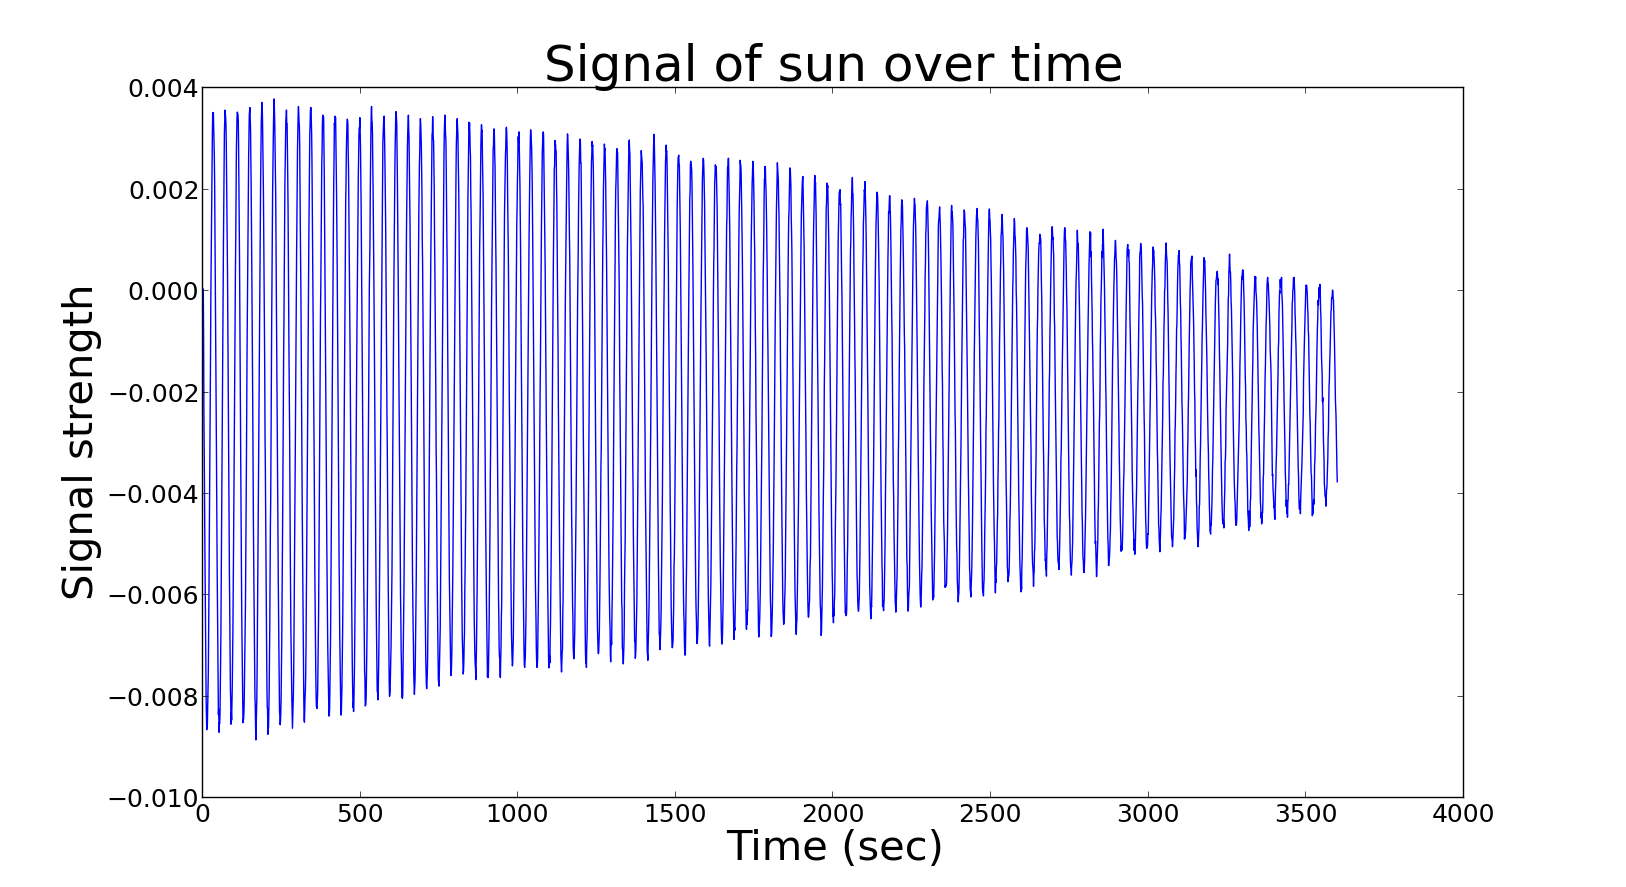
\includegraphics[scale=0.35]{garphs/sunhourvolt}
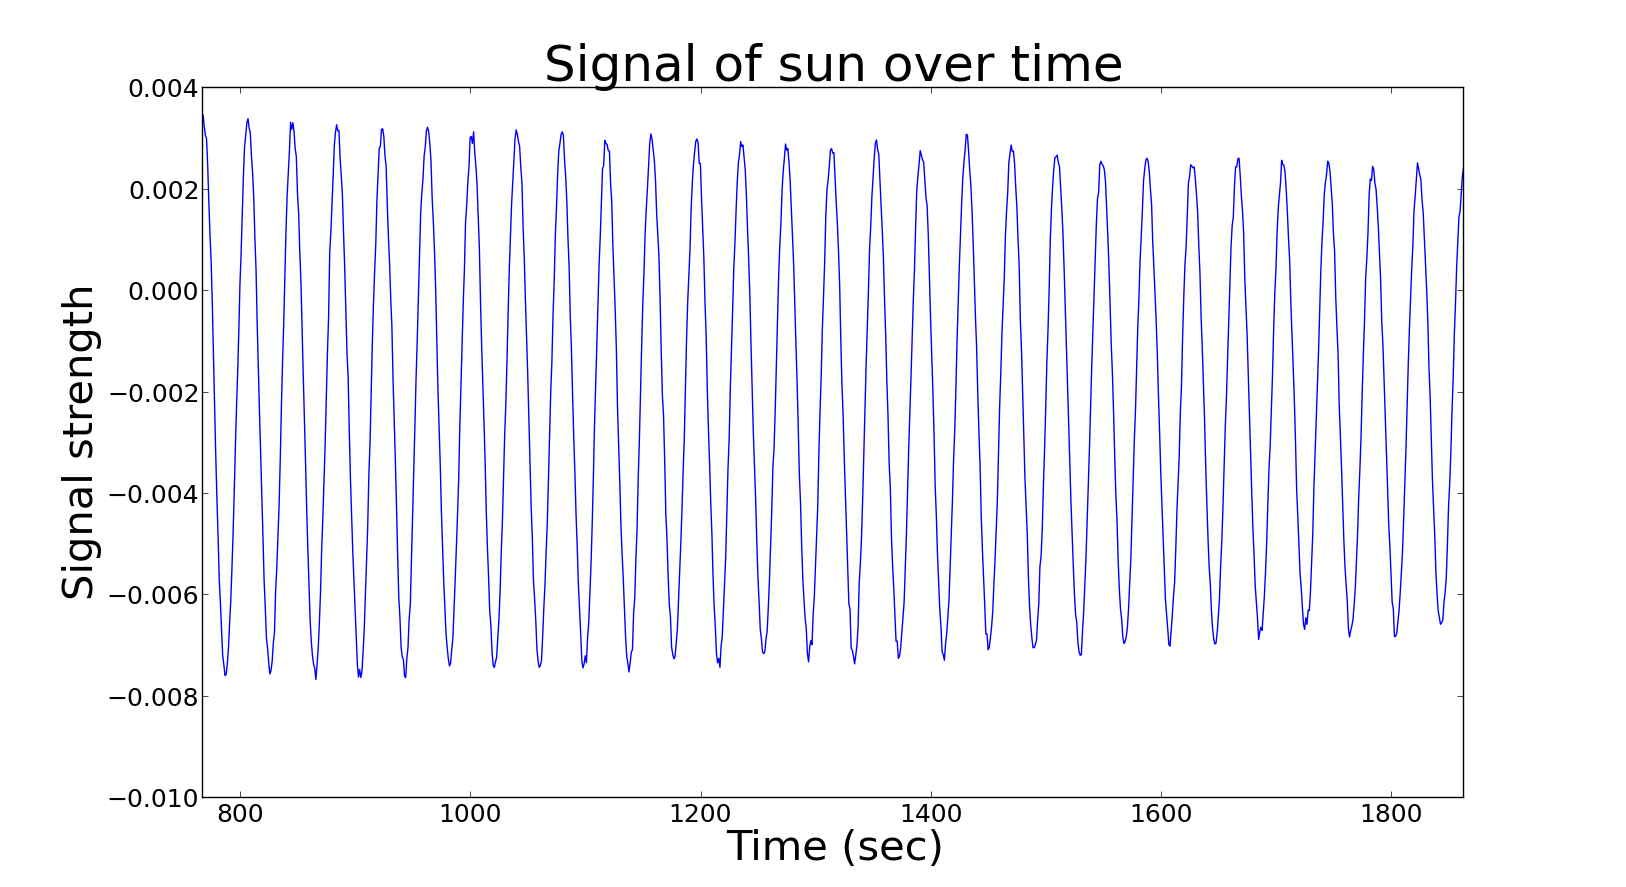
\includegraphics[scale=0.35]{garphs/sunhourzoom}
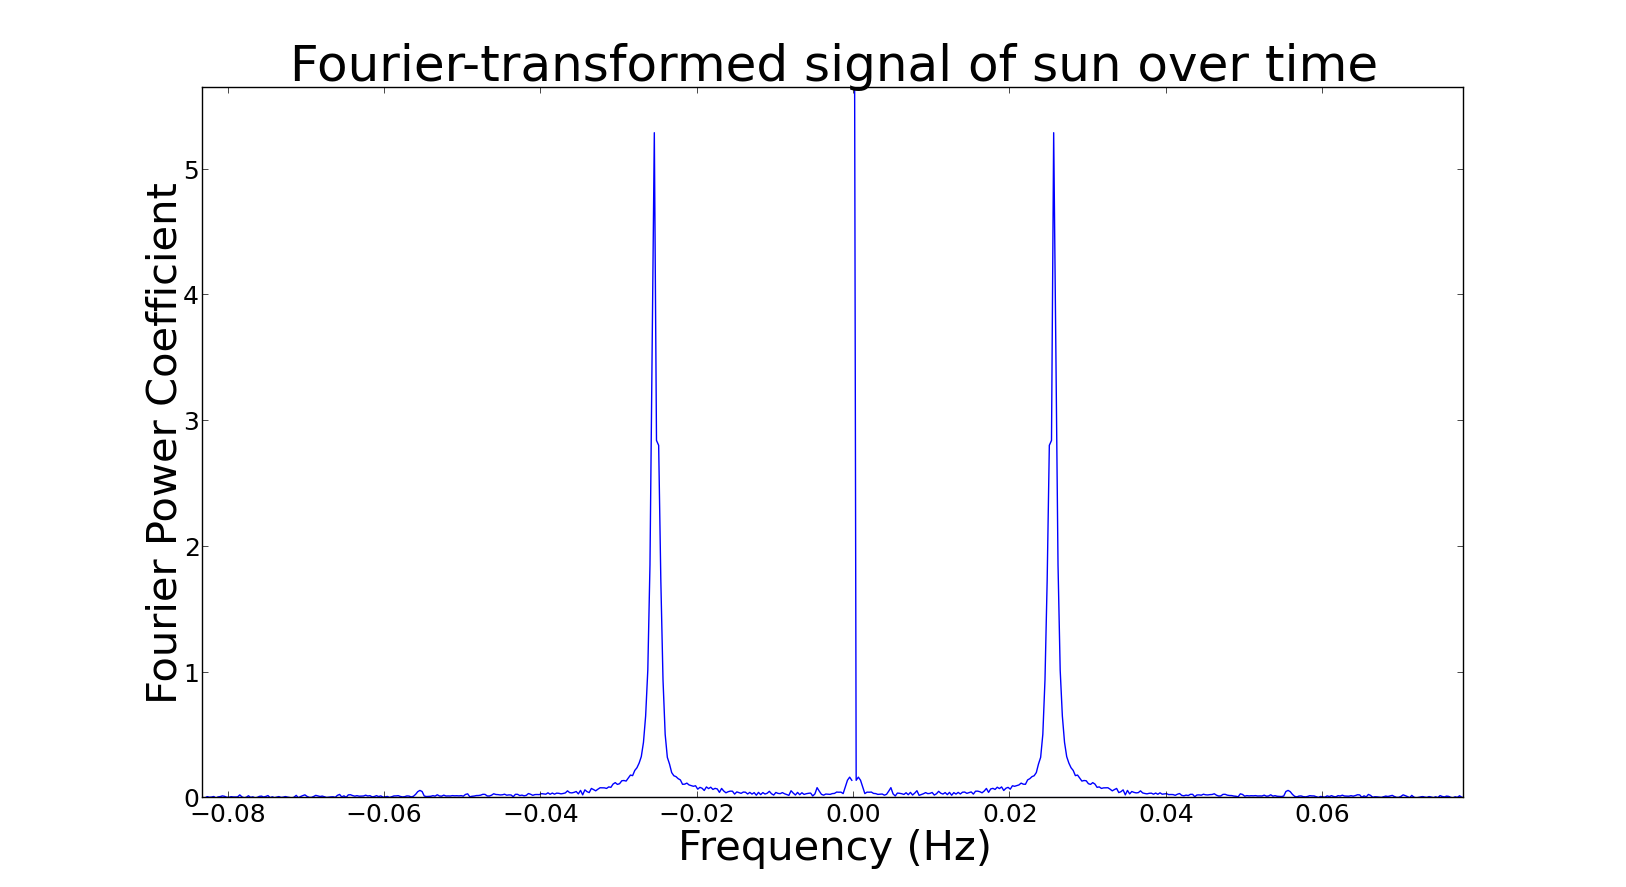
\includegraphics[scale=0.35]{garphs/sunhourfourier}
\caption{The top graph shows the signals we measured from the sun over an hour. The middle shows a zoomed-in version of this data. The bottom shows the Fourier transform of the top. \label{hoursun}}
\end{figure}

\begin{figure}
\centering
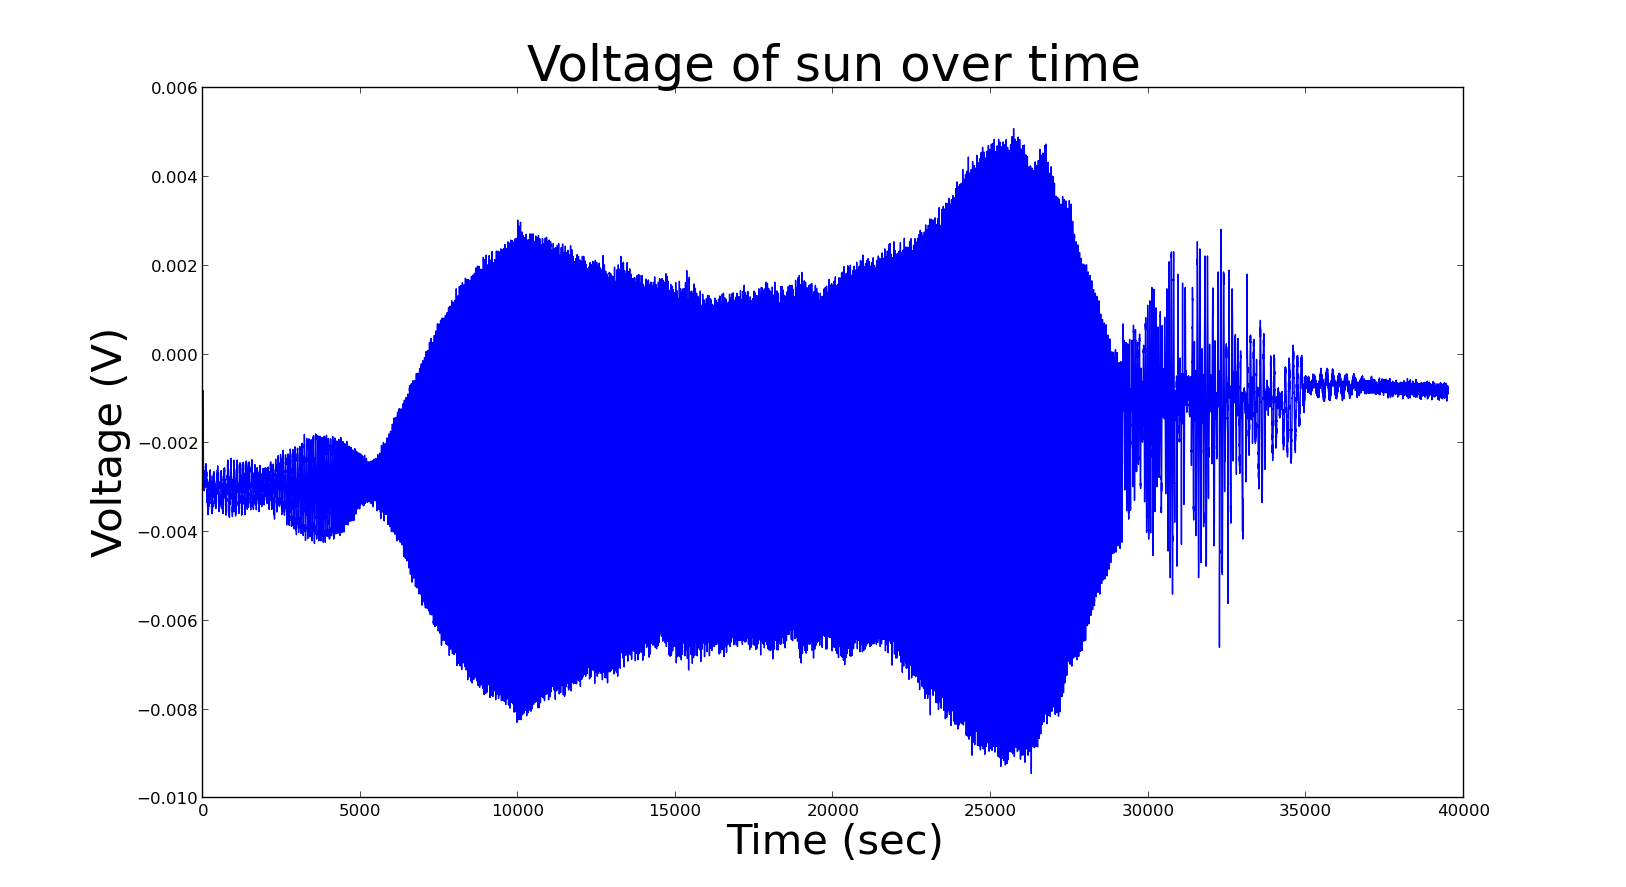
\includegraphics[scale=0.35]{garphs/sundayvolt}
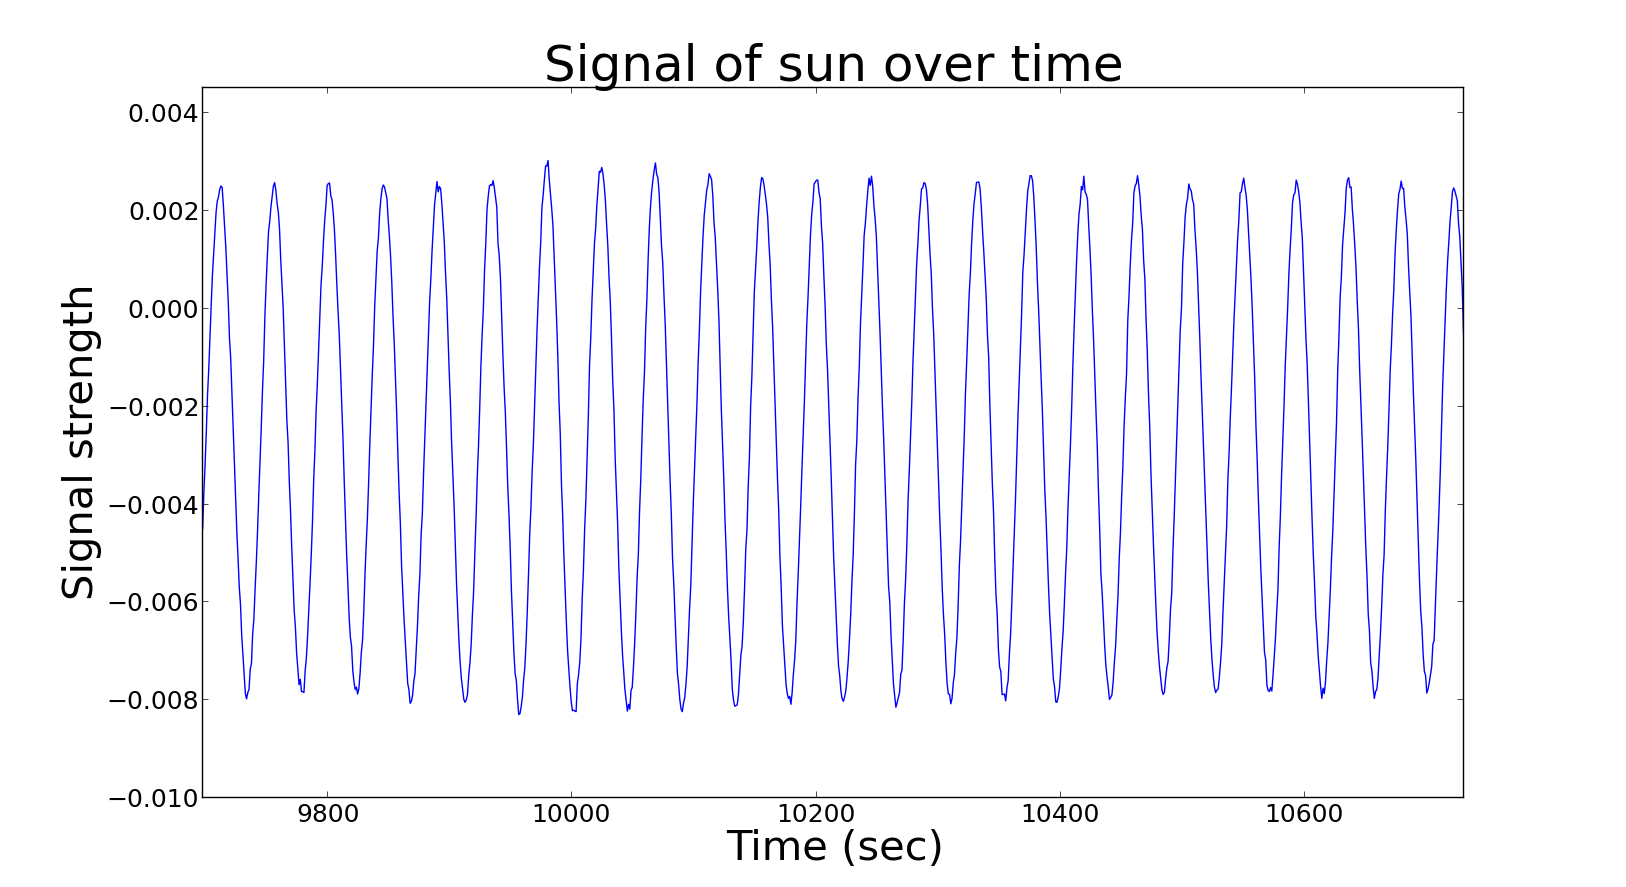
\includegraphics[scale=0.35]{garphs/sundayzoom}
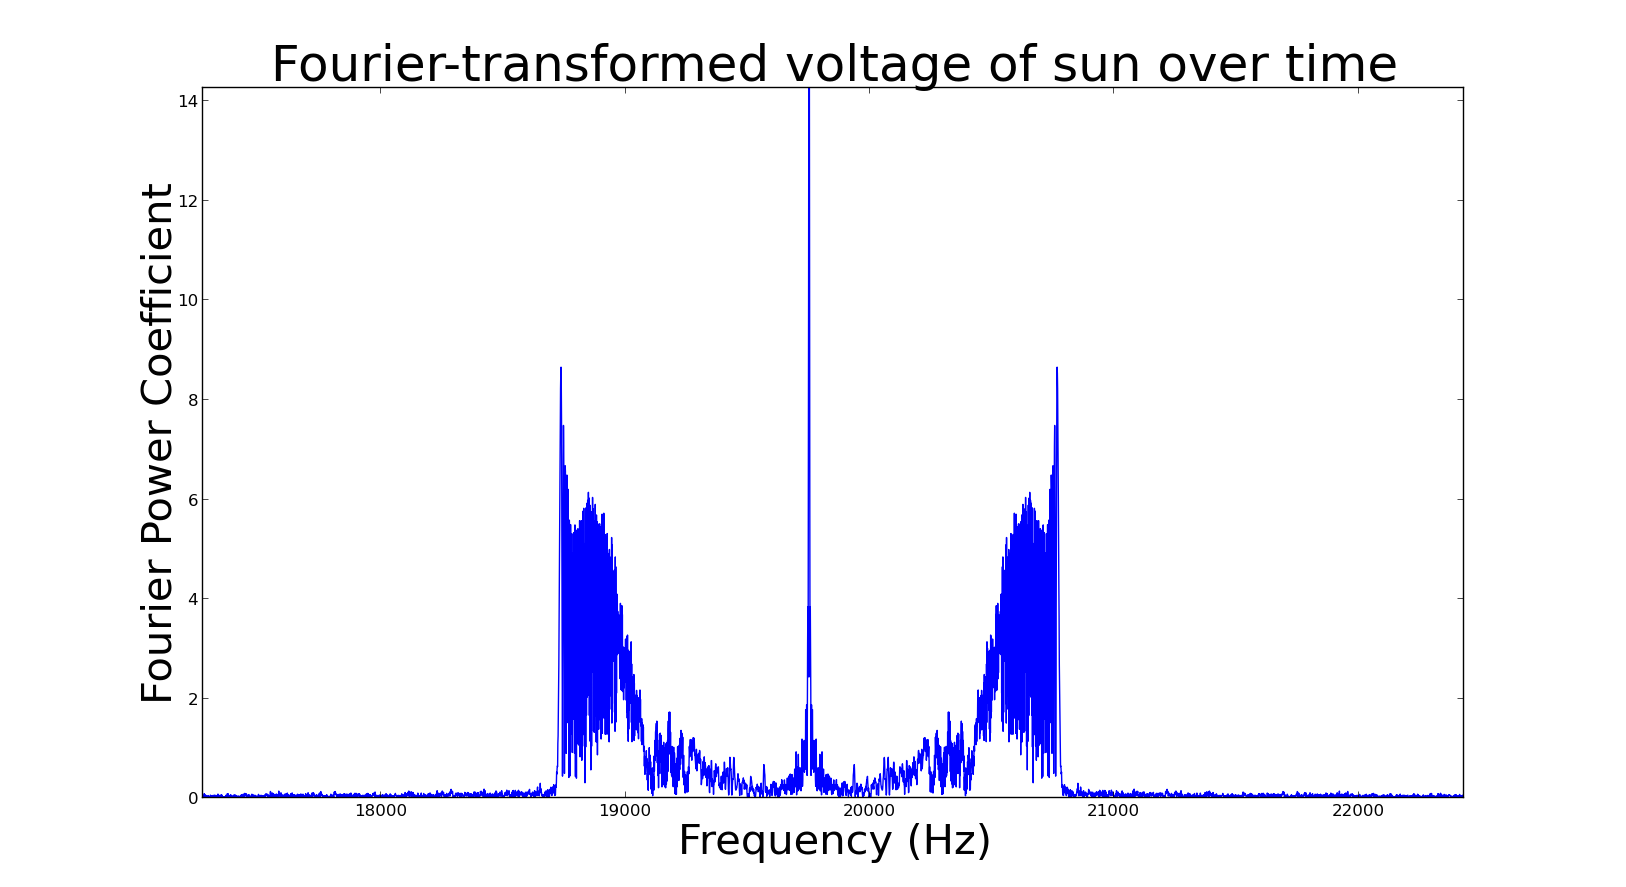
\includegraphics[scale=0.35]{garphs/sundayfourier}
\caption{The top graph shows the signals we measured from the sun over a day. The middle shows a zoomed-in version of this data. The bottom shows the Fourier transform of the top. \label{daysun}}
\end{figure}

The sun's signal comes through as a sinusoid, as we expect from the properties of the interferometer. Looking at the Fourier transform, one can see strong peaks a few thousand Hz past the DC offset in the center. As in the last lab, our Fourier distributions are symmetric about zero due to the complex exponential multiplication that the interferometer does. Using formula 11, we can calculate the expected range of fringe frequencies and compare it with our observed frequencies. Assuming $B_y = 10$m and $\lambda = 2.5$cm, we get $f_f = B_y / \lambda * 2\pi / (86400) = .03\cos{h_s}$ Hz, where $h_s$, the hour angle, varies between $-\pi/2$ and $\pi/2$ throughout the day, being 0 at the meridian. Thus, we can expect that we will see frequencies in the Fourier spectrum between 0 and $.03$ Hz, with the power increasing as we move towards .03, since the sun is strongest at the meridian. This is exactly what we see in the full-day data, and the hour-long data, which was taken around midday, just shows a strong peak around .03 Hz. \\
Then, we calculated the sun's diameter using the data. To do this, we focused specifically on the range in the first graph of Figure \ref{daysun} between 4500 and 6000, where the envelope is clearly a parabola: the minimum of this parabola corresponds to a zero of the Bessel function that we are looking for. First, we measured the phase offset of the fringe by least squares, fitting to the equation $F(h_s) = \cos({B_y / \lambda * \cos{\delta} * \cos{h_s + \phi}})$, where $F$ is the fringe amplitude, $B_y$ is the baseline, $\lambda$ is the wavelength, $h_s$ is the hour angle, and $\phi$ is the phase offset. By guessing various values of $\phi$ and finding which one fit the data best, we found $\phi$ = 3.186 rad; the relevant graph appears in Figure \ref{sunchiangle}. The equation for this parabola is $f(x) =147.6 - 53.53 x + 4.89 x^2$. Its minimal value is at 5.473, so this is the hour angle at which we will be checking for zeros. The fringe frequency $f_f$ corresponding to this hour angle is 236.9 cycles per radian. Plugging this frequency into Equation 19, guessing values for the angular size, and setting the resulting sum equal to zero, we generate the graph shown in Figure \ref{sunrad}. The points where the graph is zero correspond to potential angular sizes for the sun. So the angular size of the sun could be around 0.002 radians, 0.004 radians, 0.0065 radians, or some other zero of the function. The reference value of the angular size is roughly 16 arcminutes, which is close to the 0.004 radian value.

\begin{figure}
\centering
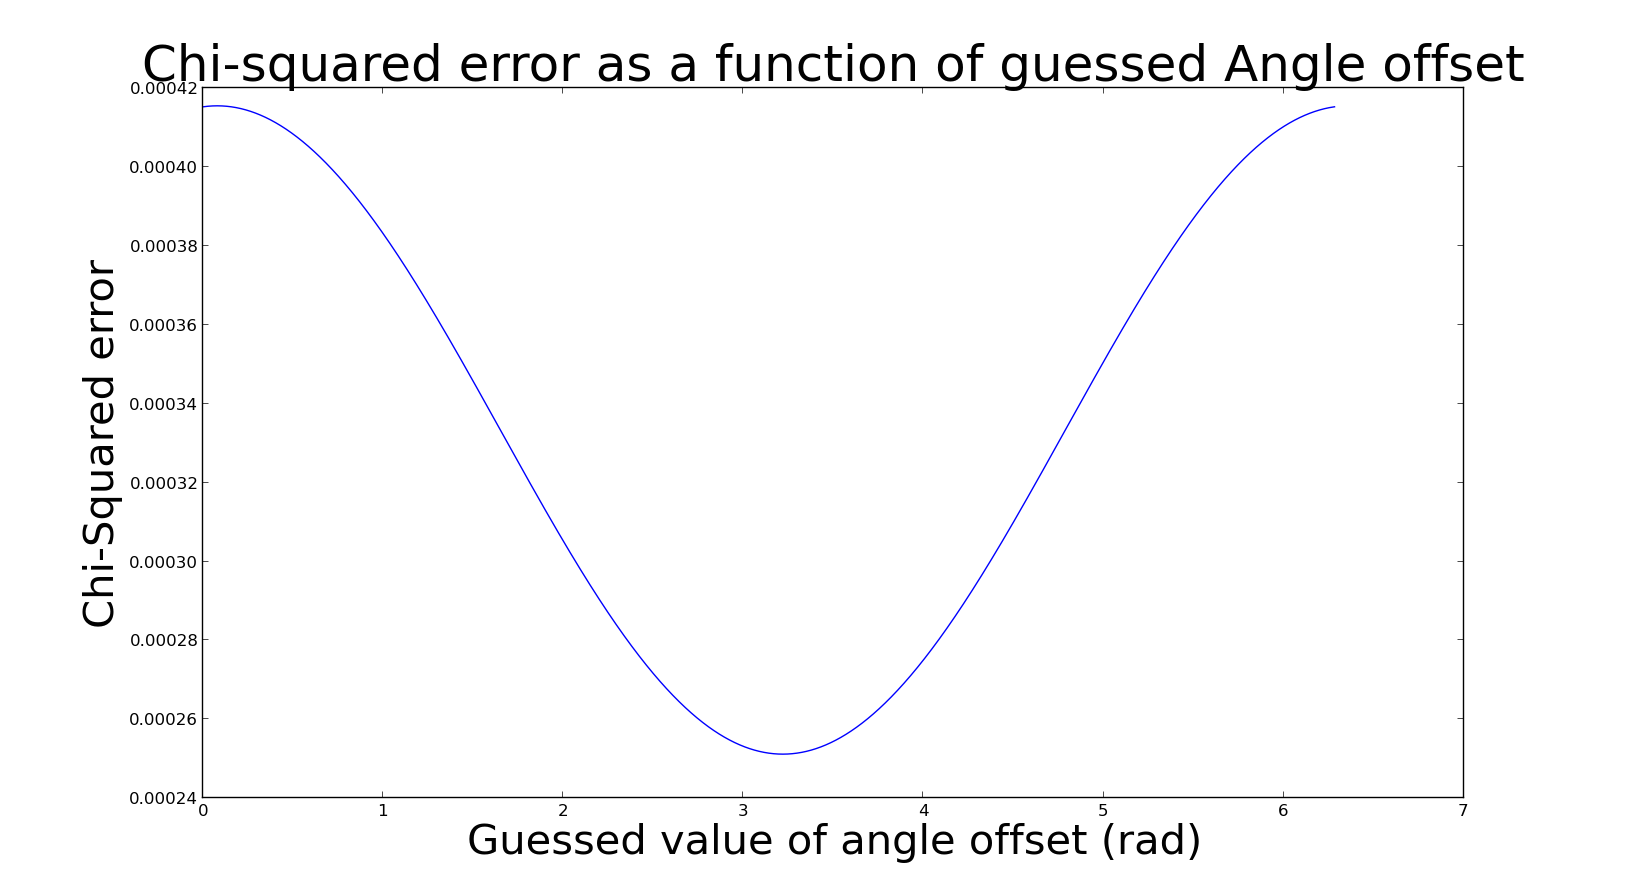
\includegraphics[scale=0.35]{garphs/sunchiangle}
\caption{The chi-squared error in our fit of the sun's radiation as a function of our guessed angle offset. \label{sunchiangle}}
\end{figure}

\begin{figure}
\centering
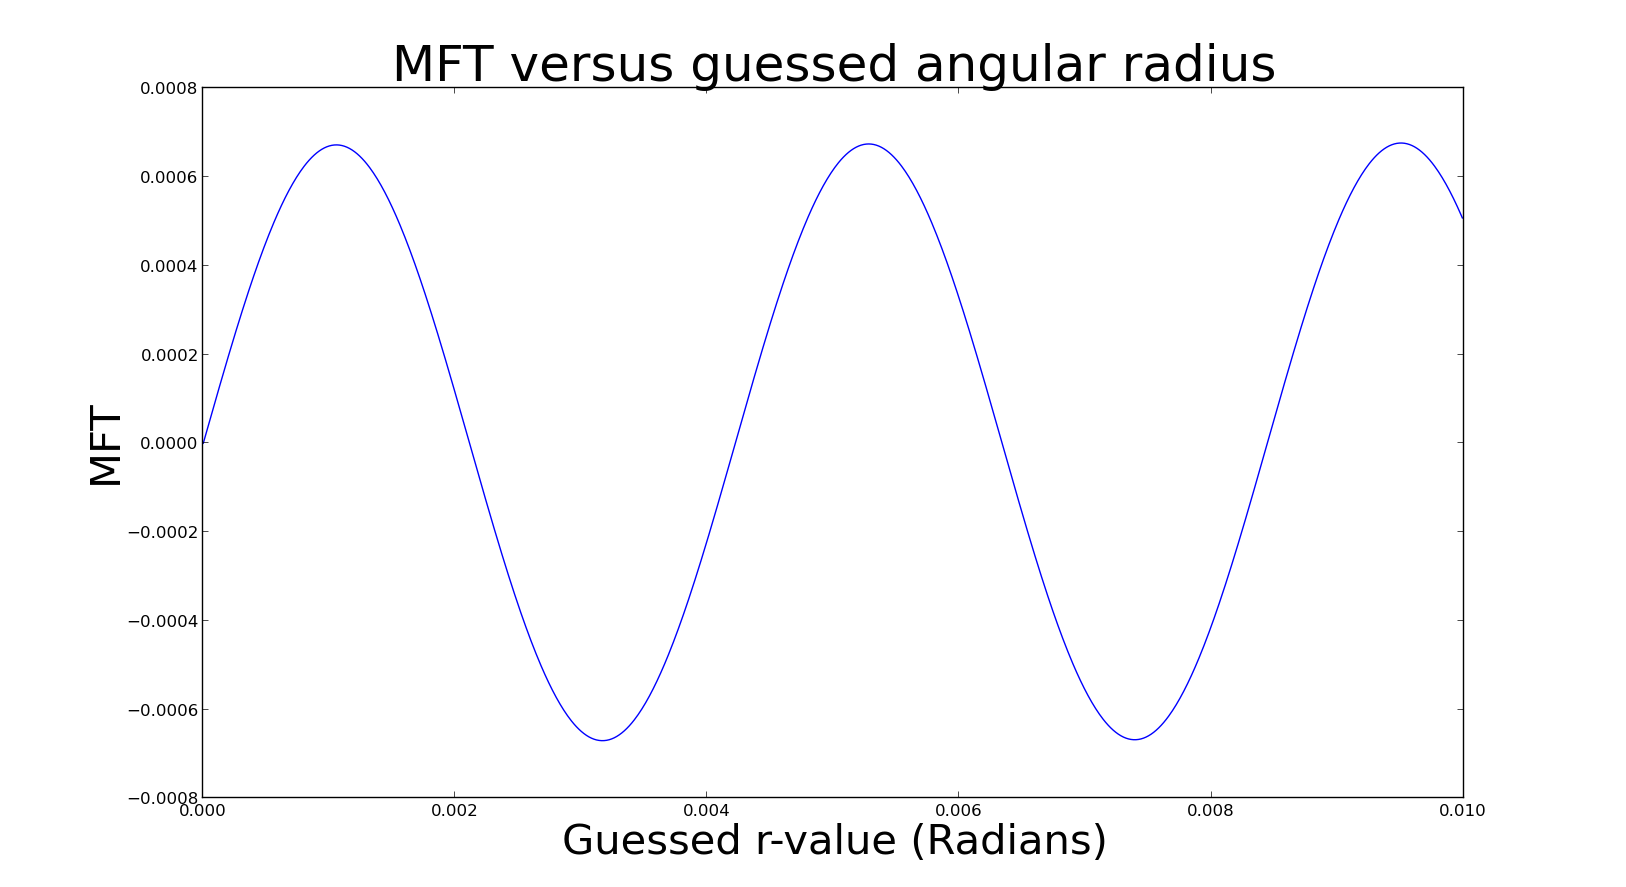
\includegraphics[scale=0.35]{garphs/sunmft}
\caption{The modulating function of the sun at 236.9 cycles per radian, as a function of guessed angular size. \label{sunrad}}
\end{figure}
\subsection{The Moon}
Then, we did all the exact same things on the moon, except we skipped the part with the hour measurements because we believed in our system already. The resulting signal and Fourier transform data appear in figure \ref{moon}.

\begin{figure}
\centering
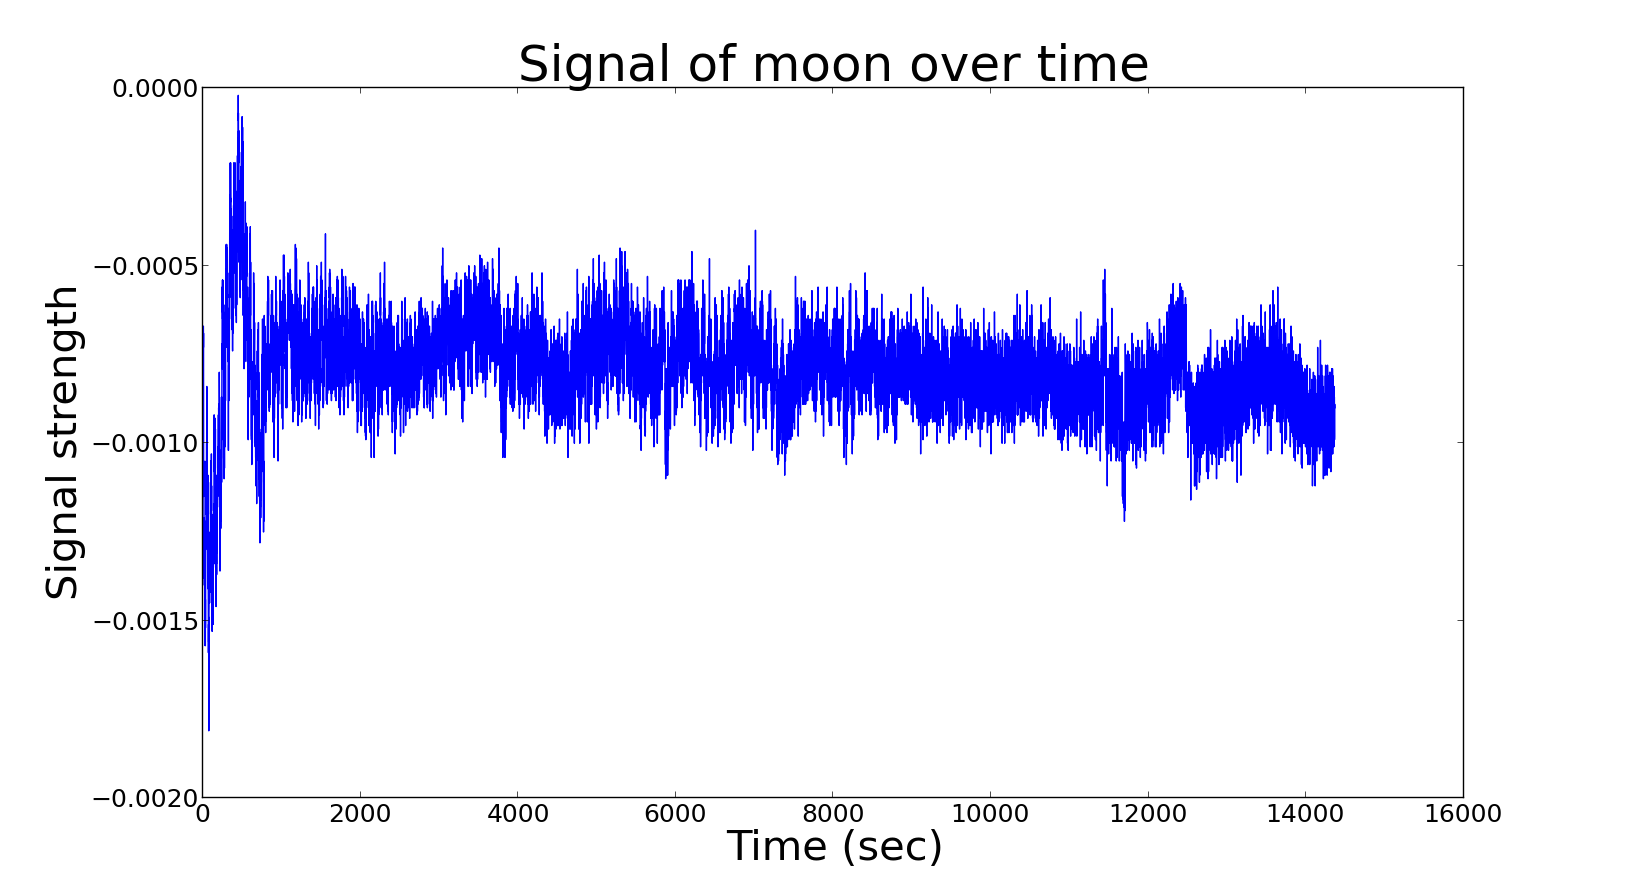
\includegraphics[scale=0.35]{garphs/moonvolt}
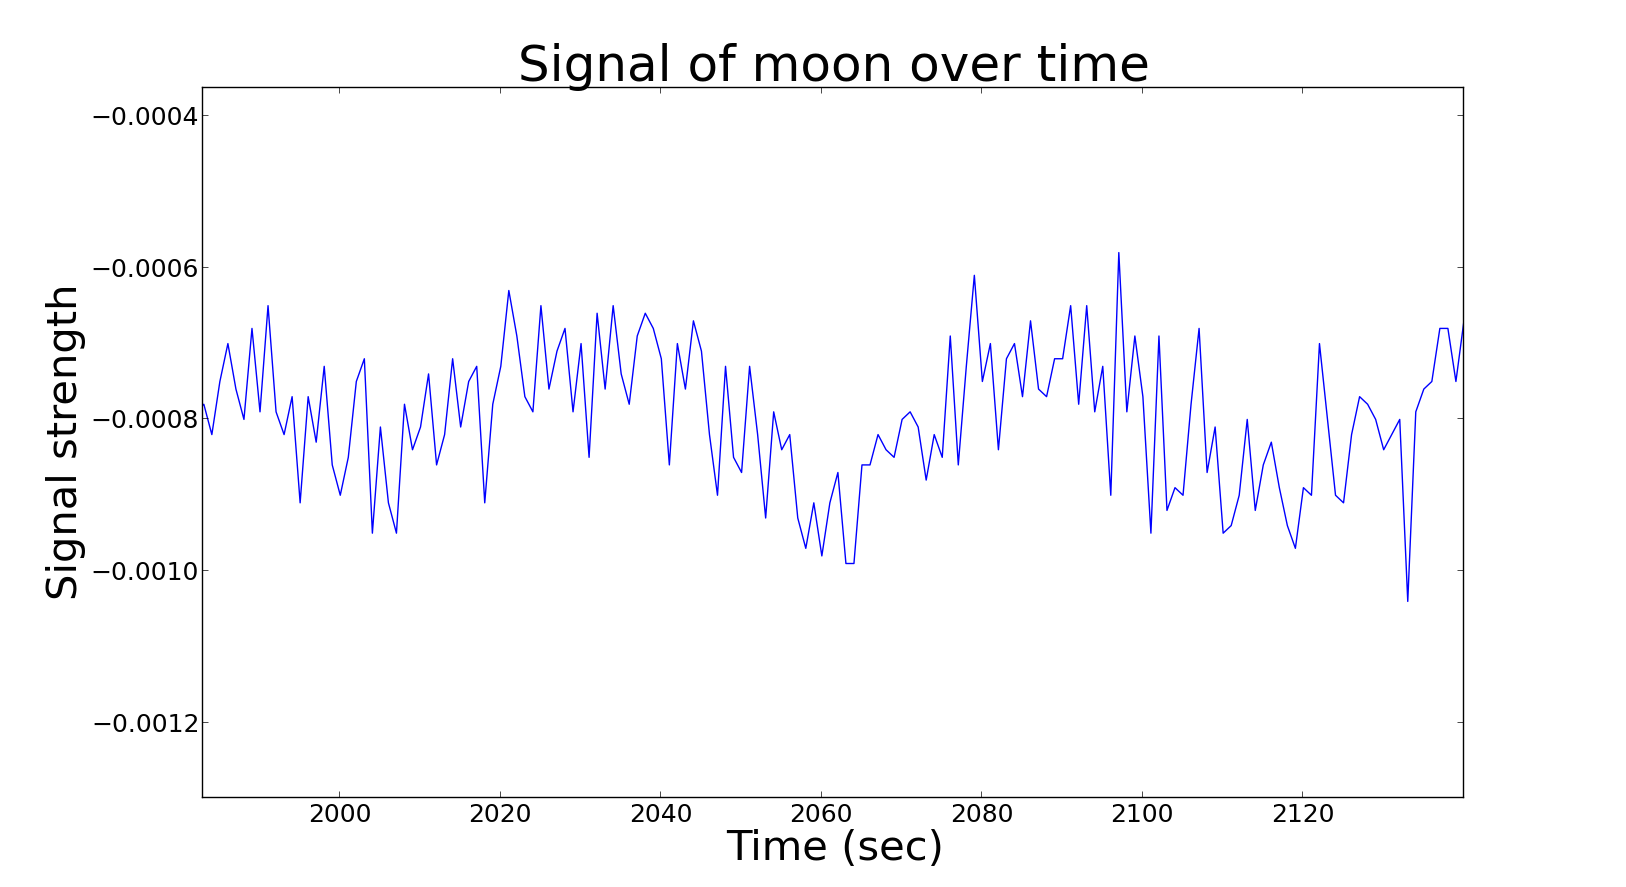
\includegraphics[scale=0.35]{garphs/moonzoom}
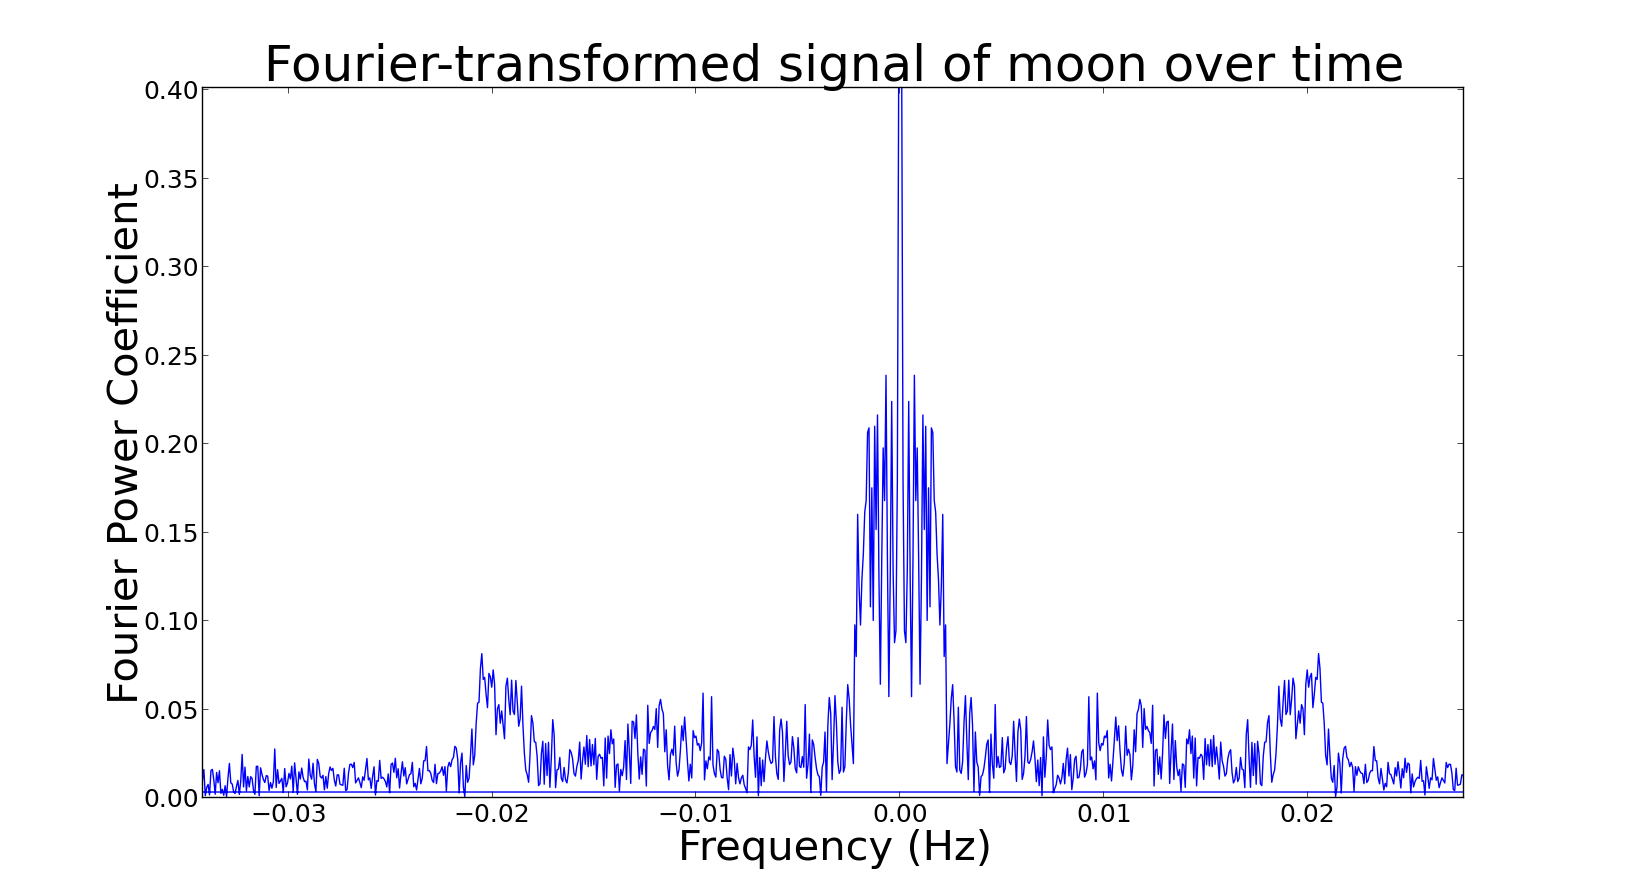
\includegraphics[scale=0.35]{garphs/moonfourier}
\caption{The top graph shows the signals we measured from the moon over several hours. The middle shows a zoomed-in version of this data. The bottom shows the Fourier transform of the top. \label{moon}}
\end{figure}

The moon radiates much more weakly than the sun, because it is a large hunk of cheese instead of a ball of fusing plasma, so its blackbody radiation is not as strong. Nevertheless, looking at the Fourier transform data, one can see unmistakable peaks in the range between 0 and 0.3 Hz, just where we would expect them to be. The fringe frequency range is the same as that for the sun because it is a property of the interferometer independent of the source. 

Then, we calculated the moon's diameter using the data. To do this, we focused specifically on the range in the first graph of Figure \ref{moon} between 1700 and 3200, where the envelope is most closely a parabola: the minimum of this parabola corresponds to a zero of the Bessel function that we are looking for. But the moon data is very noisy, so first we filtered out the high- and low-frequency noise using a Fourier filter; the resulting data appears in Figure \ref{moonfilt}. Then we measured the phase offset of the fringe by least squares, fitting to the equation $F(h_s) = \cos{B_y / \lambda * \cos{\delta} * \cos{h_s + \phi}}$, where $F$ is the fringe amplitude, $B_y$ is the baseline, $\lambda$ is the wavelength, $h_s$ is the hour angle, and $\phi$ is the phase offset. By guessing various values of $\phi$ and finding which one fit the data best, we found $\phi$ = 2.619 rad; the relevant graph appears in Figure \ref{moonchiangle}. The equation for this parabola is $f(x) =610.05 - 522.29 x + 111.7 x^2$. Its minimal value is at around 2.34, so this is the hour angle at which we will be checking for zeros. The fringe frequency $f_f$ corresponding to this hour angle is 239.98 cycles per radian. Plugging this frequency into Equation 19, guessing values for the angular size, and setting the resulting sum equal to zero, we generate the graph shown in Figure \ref{moonrad}. The points where the graph is zero correspond to potential angular sizes for the moon. So the angular size of the moon could be around 0.002 radians, 0.004 radians, 0.0065 radians, or some other zero of the function. The reference value of the angular size is roughly 16 arcminutes, which is close to the 0.004 radian value.


\begin{figure}
\centering
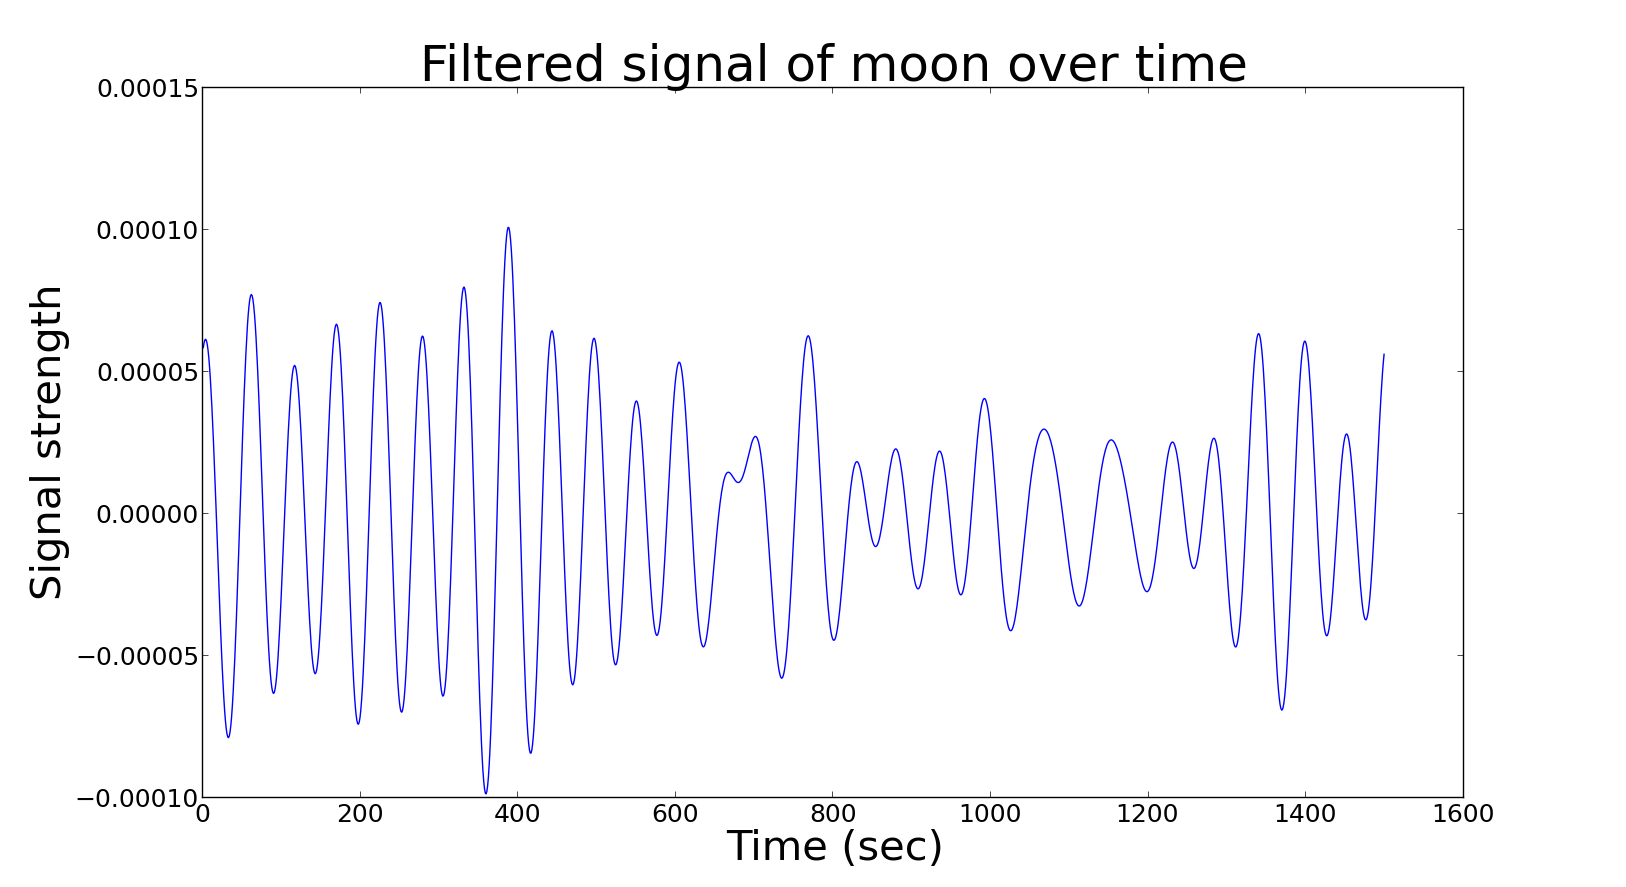
\includegraphics[scale=0.35]{garphs/filtmoon}
\caption{The signal of the moon, filtering out high- and low-frequency noise. \label{moonfilt}}
\end{figure}

\begin{figure}
\centering
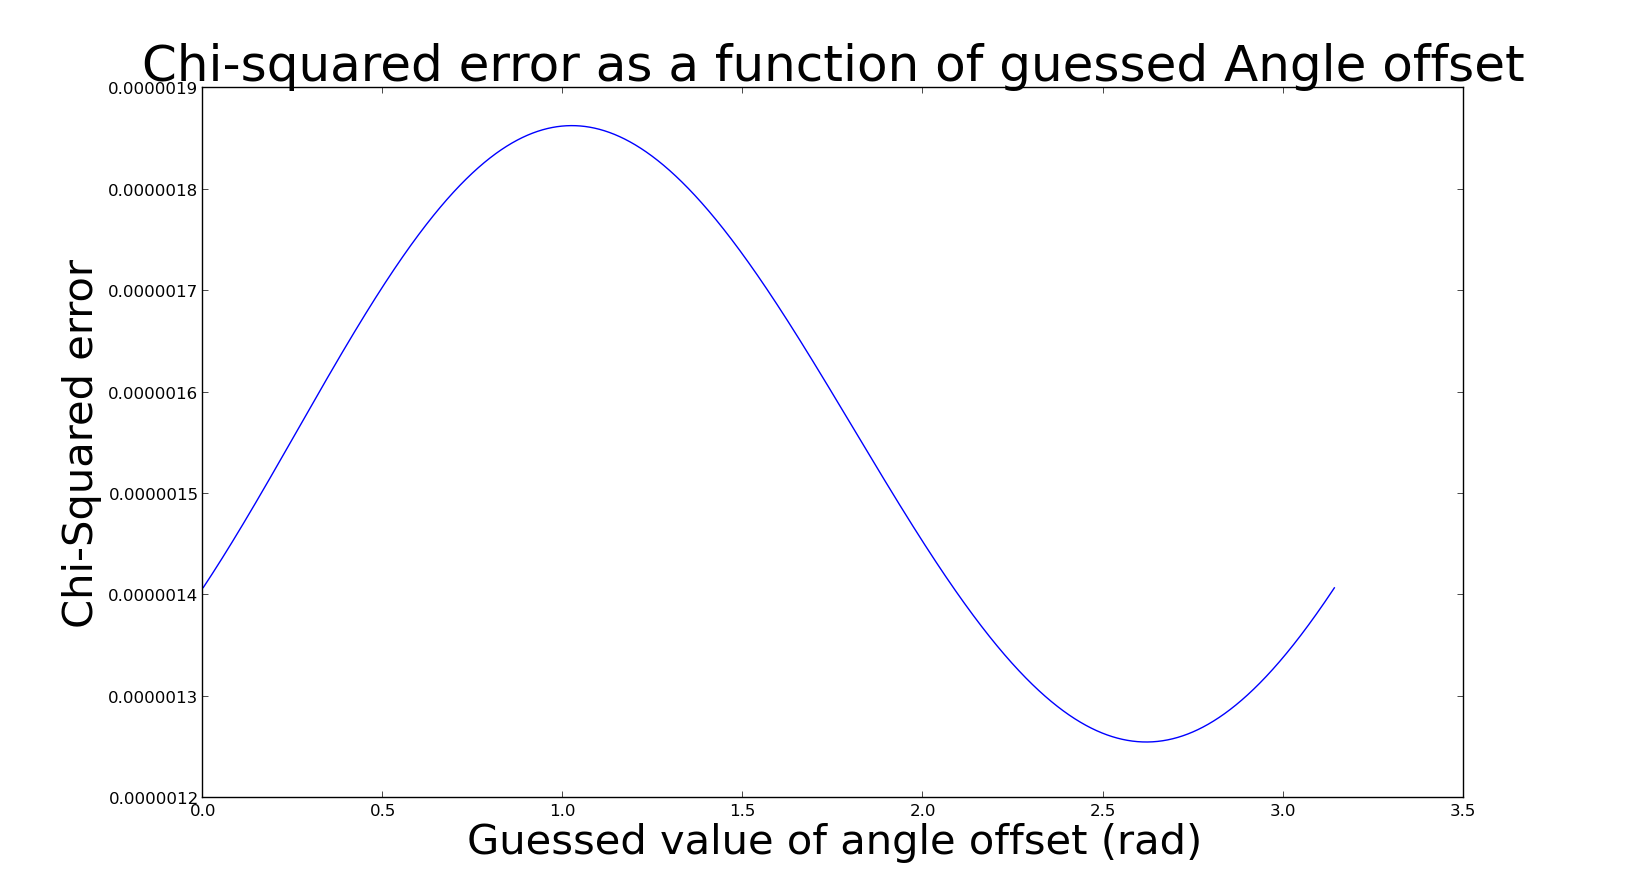
\includegraphics[scale=0.35]{garphs/moonchiangle}
\caption{The chi-squared error in our fit of the moon's radiation as a function of our guessed angle offset. \label{moonchiangle}}
\end{figure}

\begin{figure}
\centering
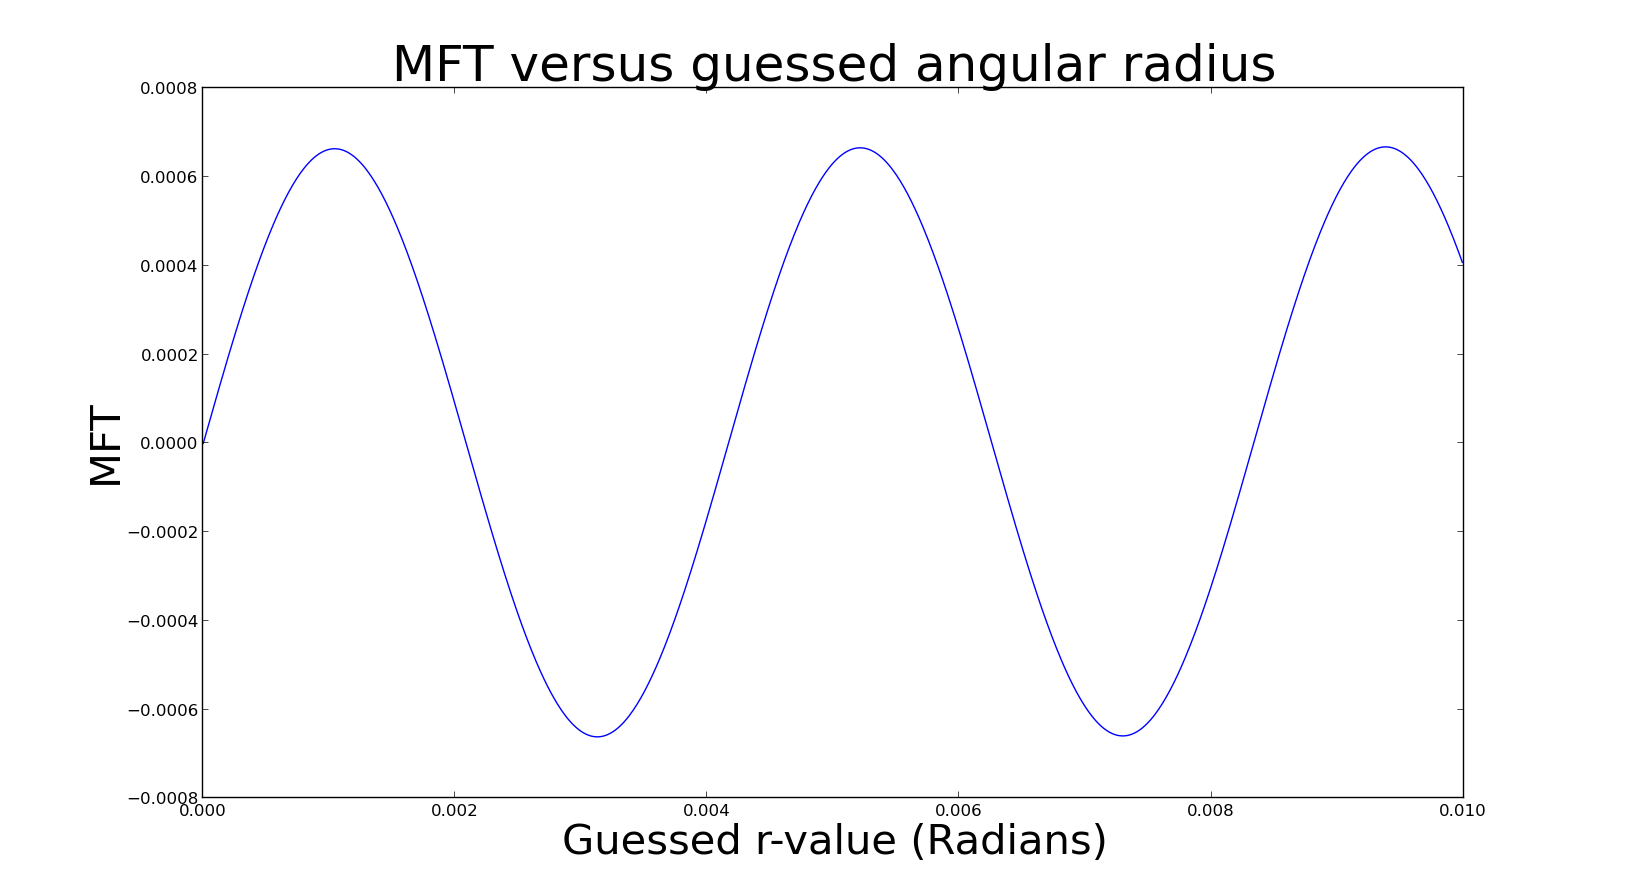
\includegraphics[scale=0.35]{garphs/moonmft}
\caption{The modulating function of the moon at 239.98 cycles per radian, as a function of guessed angular size. \label{moonrad}}
\end{figure}

\subsection{The Crab}

Finally, we looked at the Crab nebula. The signal and Fourier transform appear in Figure \ref{crab}.

\begin{figure}
\centering
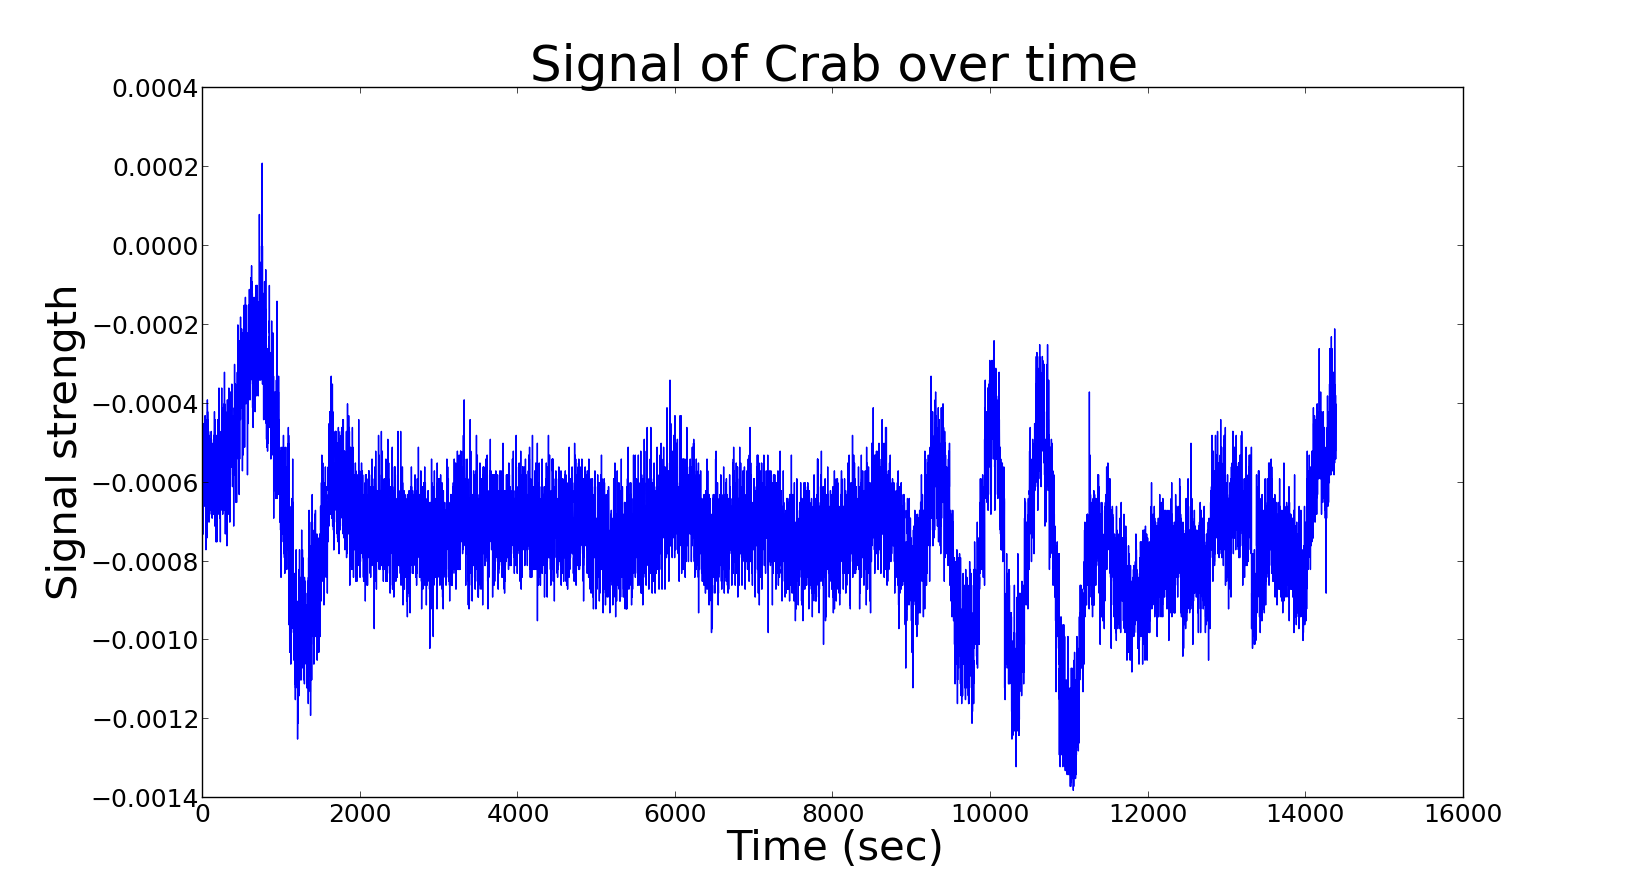
\includegraphics[scale=0.35]{garphs/crabvolt}
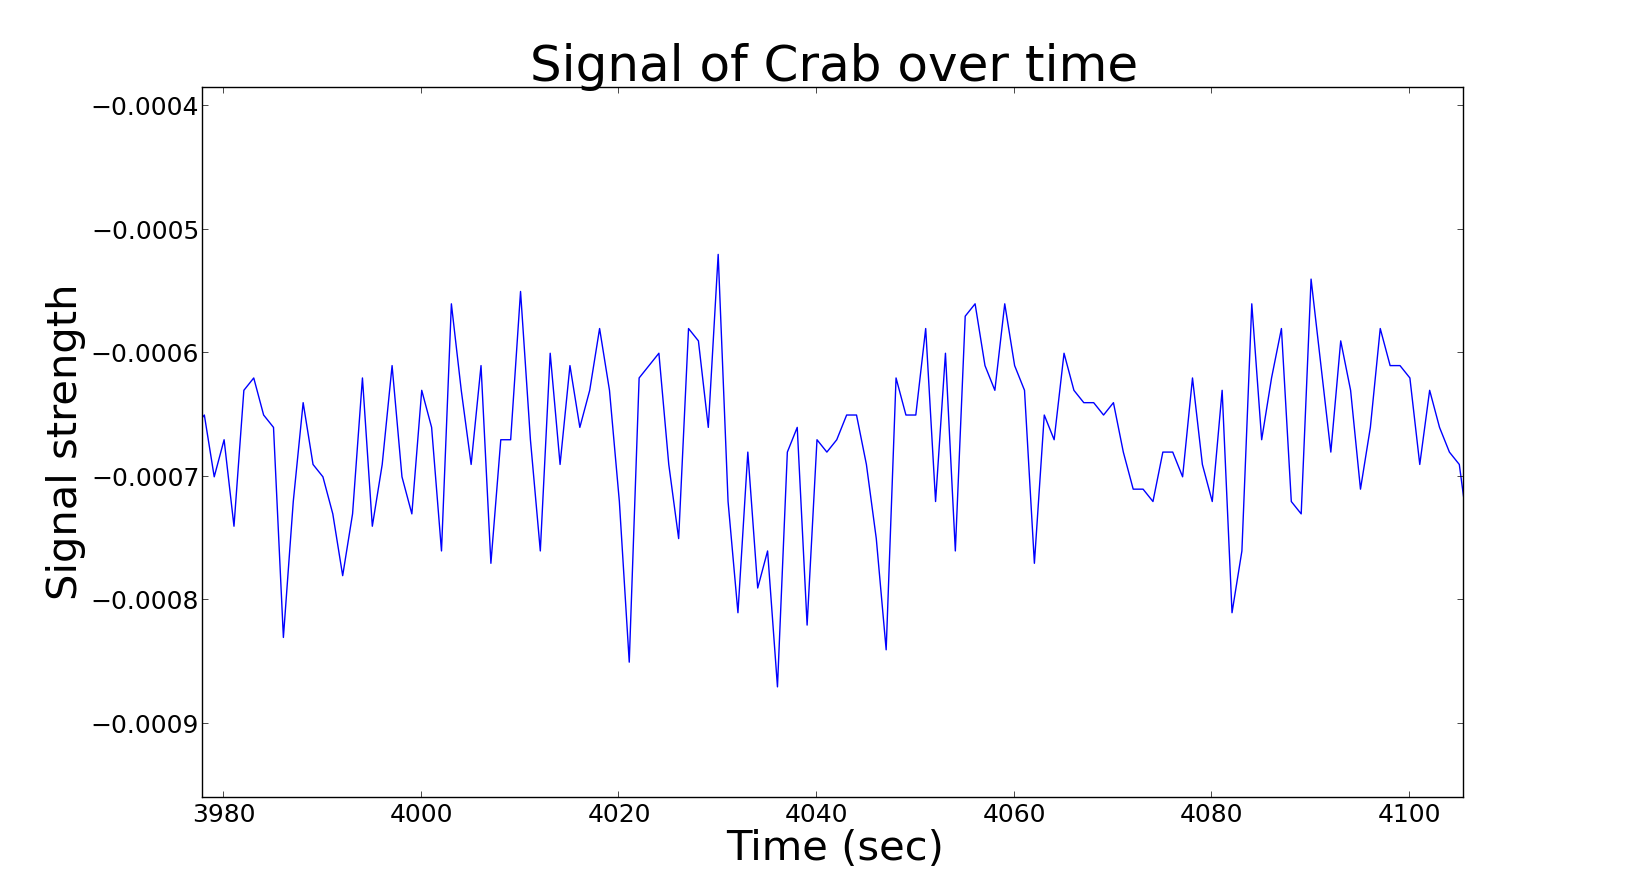
\includegraphics[scale=0.35]{garphs/crabzoom}
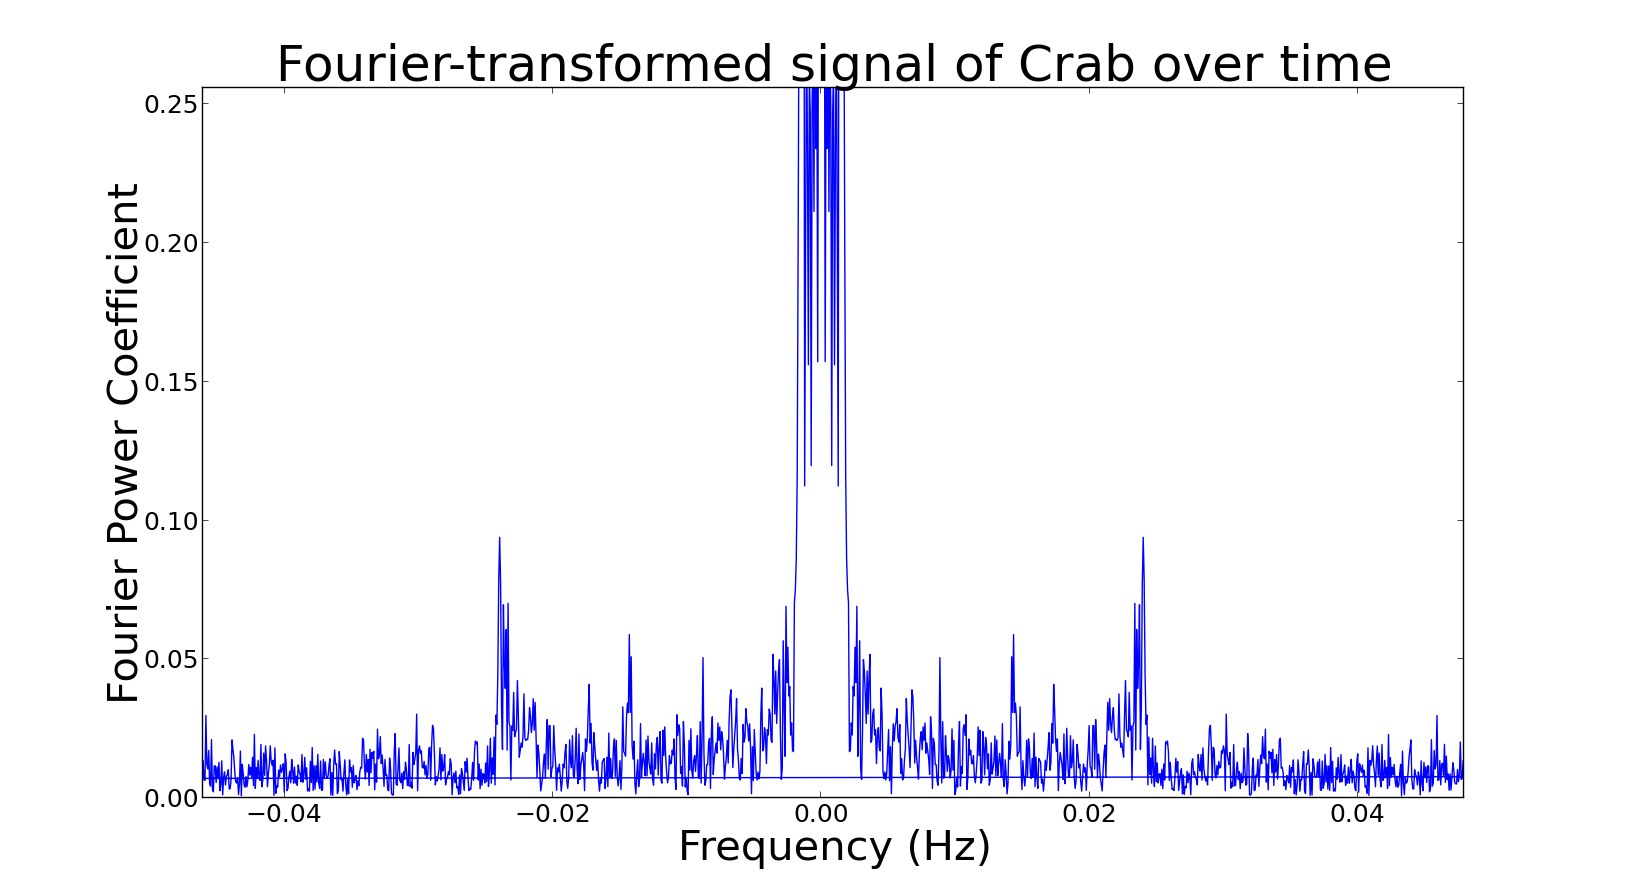
\includegraphics[scale=0.35]{garphs/crabfourier}
\caption{The top graph shows the signals we measured from the Crab nebula over several hours. The middle shows a zoomed-in version of this data. The bottom shows the Fourier transform of the top. \label{crab}}
\end{figure}

The Crab data appears similar to the moon data, having small but unmistakable peaks between 0 and 0.3 Hz, as we'd expect from such a far-off source. Using this data, we estimated the length of the telescope baseline using brute force least-squares fitting. Assuming we had accurate values of the declination and right ascension, we made guesses at the proper value of the baseline to use in equation 9. Also, we tried to fit not the data that you see in Figure \ref{crab}, but rather a smoothed, filtered version of the data as seen in Figure \ref{crabsmooth}, because the unfiltered, unsmoothed data is very noisy and incluldes effects not relevant to our measurements. Figure \ref{crabsmooth} shows the data in the top graph of Figure \ref{crab}, with a Fourier filter applied to cut out frequencies lower than 0.01 Hz or greater than 0.0203 Hz and a boxcar smooth applied to remove the envelope variation and center the data about 0. The 0.01 Hz value on the Fourier filter was chosen because that corresponds to a baseline length of around 6 meters, which is clearly too short; the .0203 corresponds to a a baseline length of around 12 meters, which is clearly too long. The boxcar smooth subtracted from each point of the original data the median of the ten measurements surrounding that point. A plot of the measured chi-square error versus the guessed values of baseline length appears in Figure \ref{crabchi}.

\begin{figure}
\centering
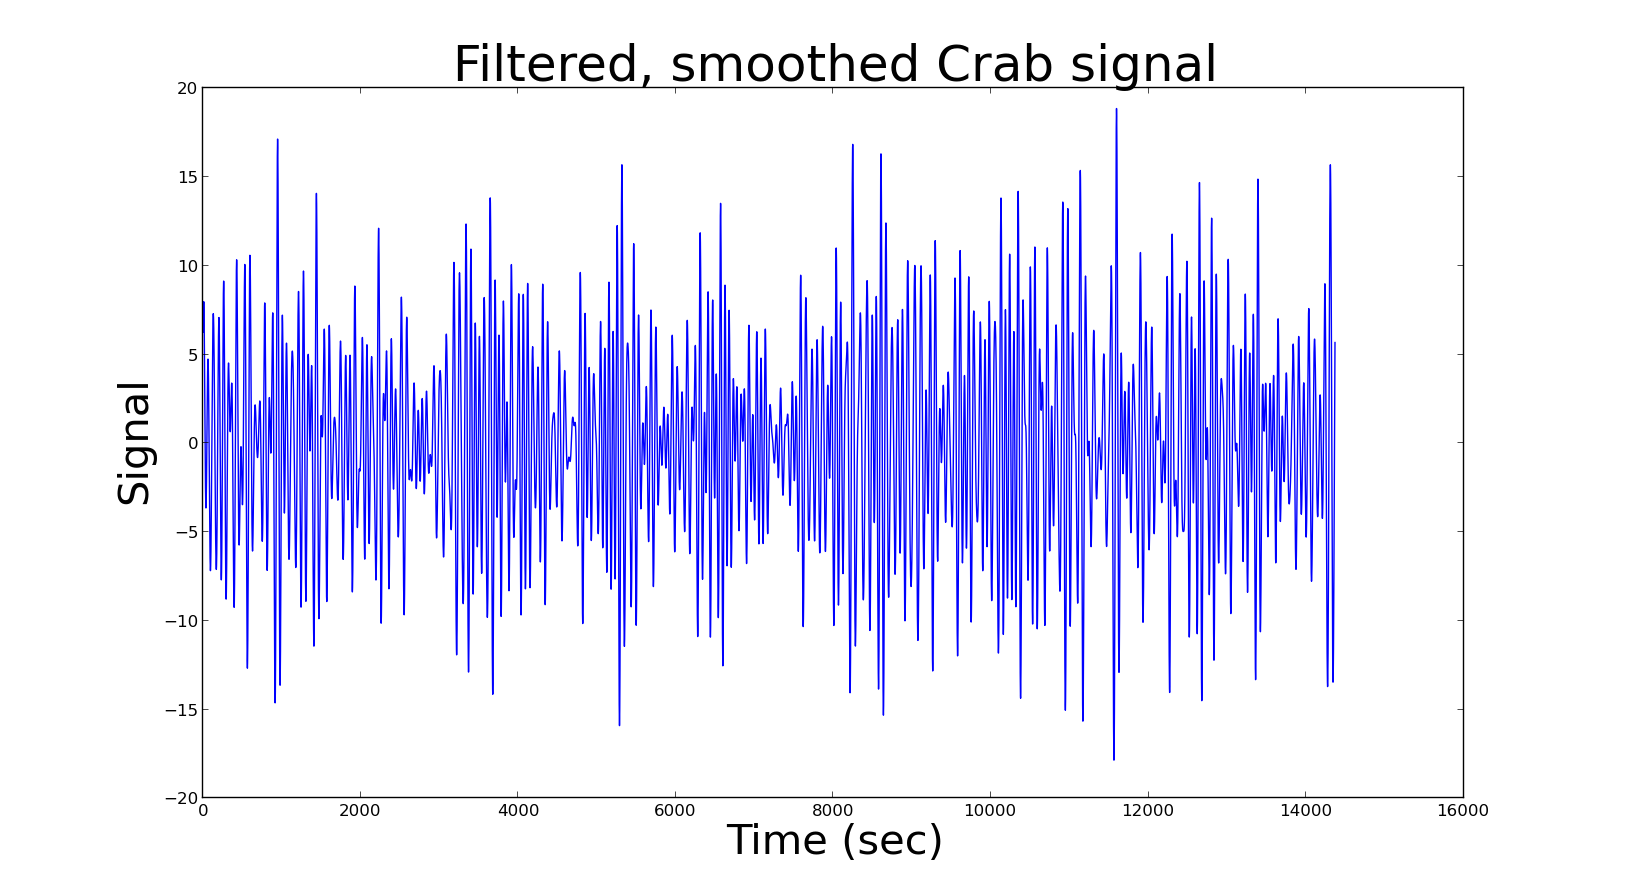
\includegraphics[scale=0.35]{garphs/crabsmooth}
\caption{ Smoothed, filtered signal of the Crab nebula. \label{crabsmooth}}
\end{figure}

\begin{figure}
\centering
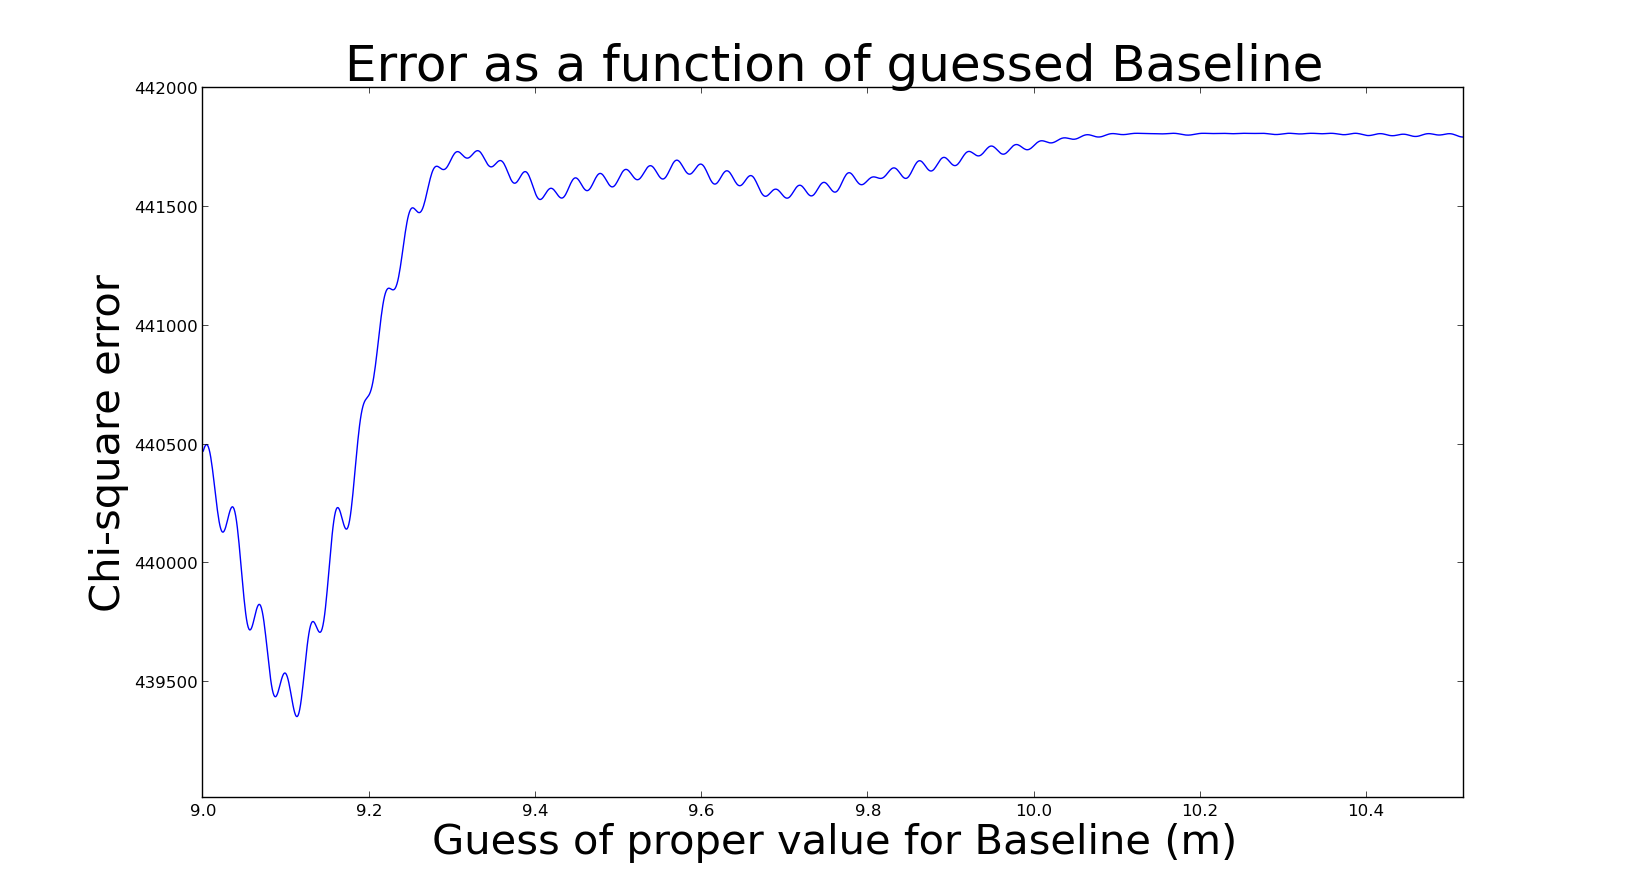
\includegraphics[scale=0.35]{garphs/crabchi}
\caption{ Error in fit of equation 9 as a function of guessed baseline length. \label{crabchi}}
\end{figure}

Our data fits best with a baseline length of around 9.1 meters. This is reasonably close to the canonical value of 10 meters, but it is not exactly there. This could have been due to noise in the data, problems with the interferometer (though our logs registered nothing), or problems with the fitting process, which seems more an art than a science. In particular, even the filtered and smoothed Crab data is still oscillating at a very high frequency, which makes it difficult to fit well. Anyway, the resulting fit is an abject failure, as depicted in Figure \ref{failure}. This value of the baseline yields values for $A$ and $B$ in equation 9 of -0.41 and 0.41, respectively. Using these values for $A$ and $B$, we find a cable length of $\cos\inv {A}  / (2 \pi\nu) = 2.65 * 10^{-2}$ nm. This cable length is shorter than anyone would think reasonable, surely because of the low quality of our fit. 

\begin{figure}
\centering
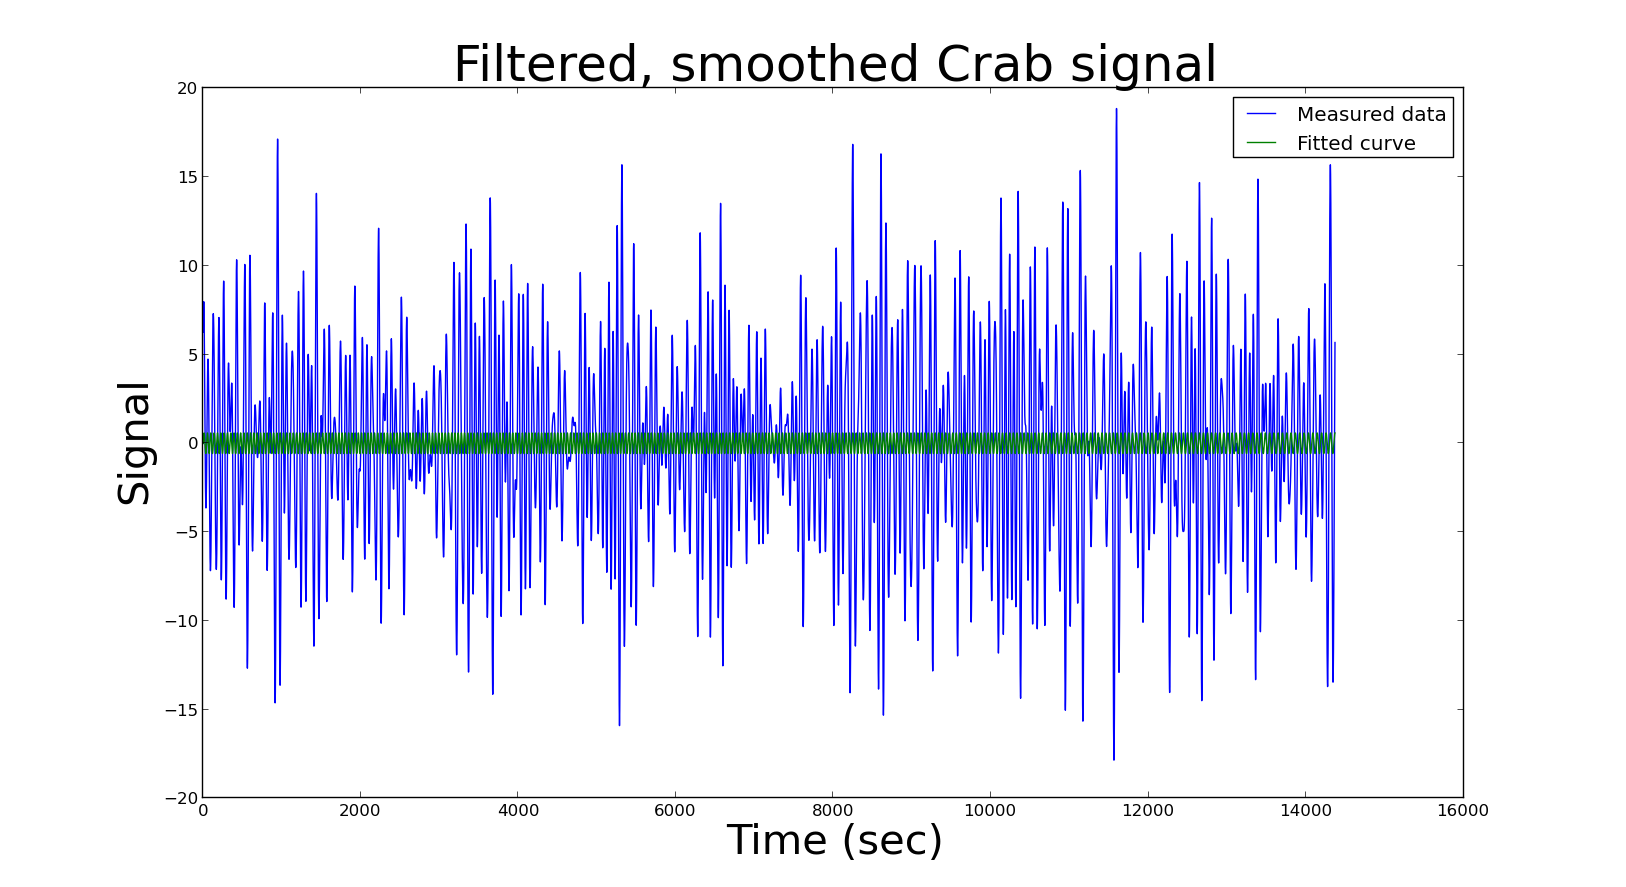
\includegraphics[scale=0.35]{garphs/failure}
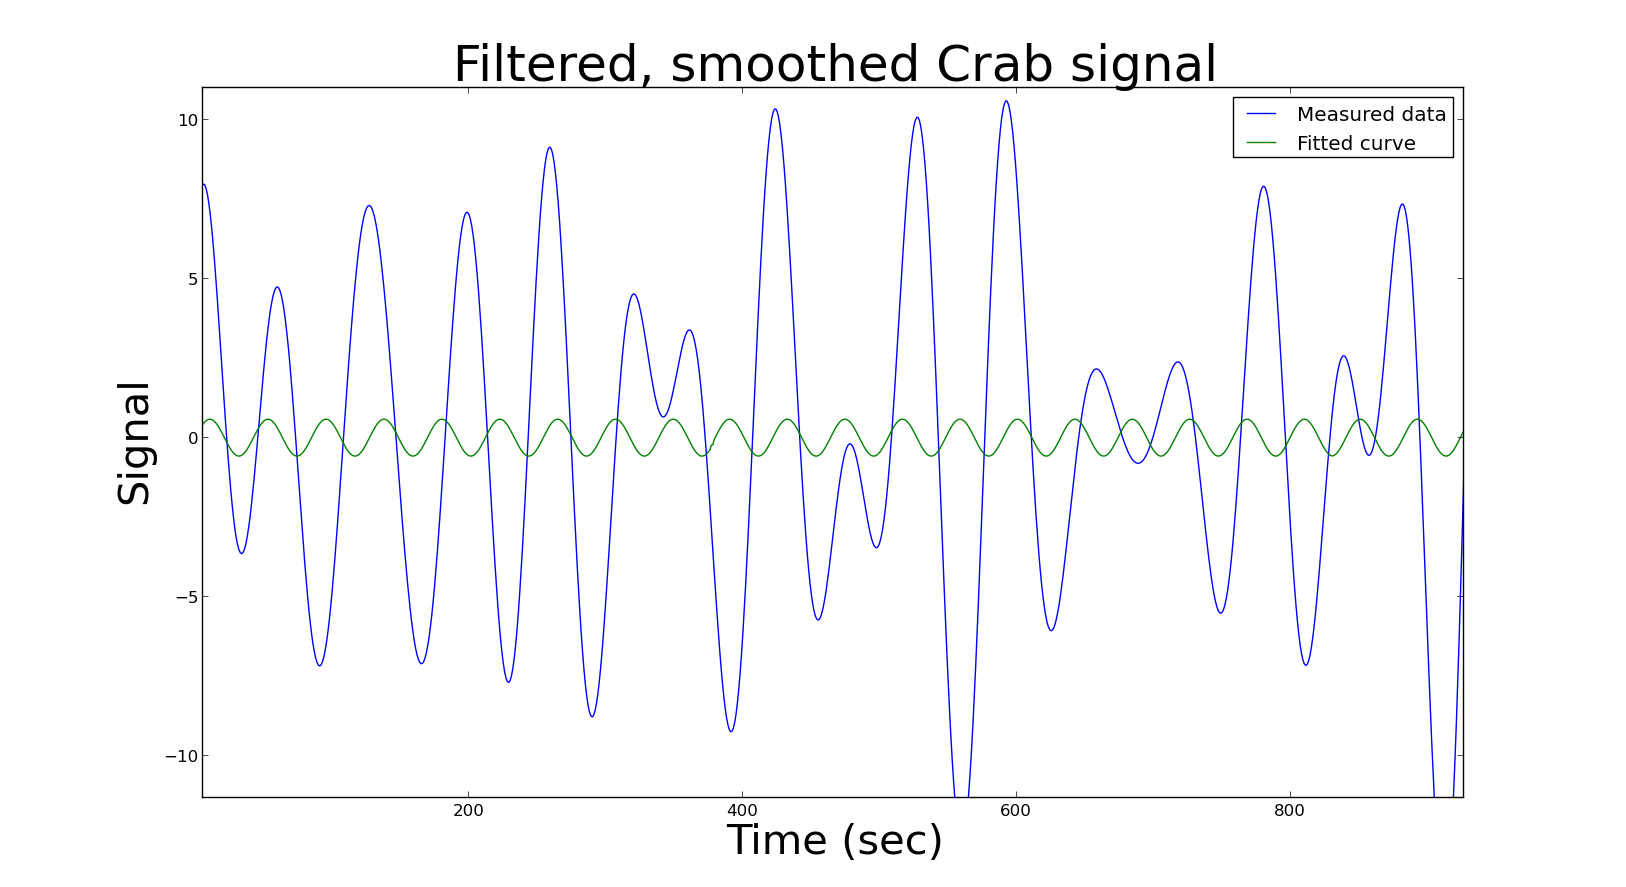
\includegraphics[scale=0.35]{garphs/failurezoom}
\caption{ A least-squares fit to the filtered, smoothed data. The top shows the whole signal, and the bottom shows a zoom-in of the early part. \label{failure}}
\end{figure}

%COMMENT: Using \label{value} and \ref{value} will allow you to refer to
%a specific figure without worrying about the order in which you have
%them in your document. While this obviously matters somewhat in terms
%of the logical flow of you paper, it's really helpful if you're moving
%things around as you write your paper. I did this for the first figure,
%but you can change the rest fairly easily. Additionally, \centering
%will put the figure in the middle of the page when you scale it down to
%a more reasonable size.

%COMMENT:By placing your figures in the flow of your text, you can
%increase the likelihood that they appear in reasonable places based on
%where you reference them. Combining figures (2 & 3 were combined) that
%are related or demonstrate two aspects of one thing can also allow you
%to use space in your paper more effectively.


%COMMENT: Captions should go below figures always.
\section{Conclusion}
In conclusion, this was a really cool lab. We measured electromagnetic radiation emanating from incredibly distant bodies, and we were able to draw some interesting conclusions about the universe based on these measurements. Given more time, we may want to look again at the signal from the Crab nebula and try to get some data that more easily fits with our model. Or we may want to look at other celestial bodies, as the sky has many things in it. I can't wait to see what we do next time!
%COMMENT: In a report you don't need to write out unit names, and it
%would actually be preferred you use things like $\mu$H versus mircoHenry
\section{Acknowledgements}
My partners were Vikram, Maissa and Marta. We made a really fantastic team!
\end{document}
